% Template for PLoS
% Version 3.5 March 2018
%
% % % % % % % % % % % % % % % % % % % % % %
%
% -- IMPORTANT NOTE
%
% This template contains comments intended 
% to minimize problems and delays during our production 
% process. Please follow the template instructions
% whenever possible.
%
% % % % % % % % % % % % % % % % % % % % % % % 
%
% Once your paper is accepted for publication, 
% PLEASE REMOVE ALL TRACKED CHANGES in this file 
% and leave only the final text of your manuscript. 
% PLOS recommends the use of latexdiff to track changes during review, as this will help to maintain a clean tex file.
% Visit https://www.ctan.org/pkg/latexdiff?lang=en for info or contact us at latex@plos.org.
%
%
% There are no restrictions on package use within the LaTeX files except that 
% no packages listed in the template may be deleted.
%
% Please do not include colors or graphics in the text.
%
% The manuscript LaTeX source should be contained within a single file (do not use \input, \externaldocument, or similar commands).
%
% % % % % % % % % % % % % % % % % % % % % % %
%
% -- FIGURES AND TABLES
%
% Please include tables/figure captions directly after the paragraph where they are first cited in the text.
%
% DO NOT INCLUDE GRAPHICS IN YOUR MANUSCRIPT
% - Figures should be uploaded separately from your manuscript file. 
% - Figures generated using LaTeX should be extracted and removed from the PDF before submission. 
% - Figures containing multiple panels/subfigures must be combined into one image file before submission.
% For figure citations, please use "Fig" instead of "Figure".
% See http://journals.plos.org/plosone/s/figures for PLOS figure guidelines.
%
% Tables should be cell-based and may not contain:
% - spacing/line breaks within cells to alter layout or alignment
% - do not nest tabular environments (no tabular environments within tabular environments)
% - no graphics or colored text (cell background color/shading OK)
% See http://journals.plos.org/plosone/s/tables for table guidelines.
%
% For tables that exceed the width of the text column, use the adjustwidth environment as illustrated in the example table in text below.
%
% % % % % % % % % % % % % % % % % % % % % % % %
%
% -- EQUATIONS, MATH SYMBOLS, SUBSCRIPTS, AND SUPERSCRIPTS
%
% IMPORTANT
% Below are a few tips to help format your equations and other special characters according to our specifications. For more tips to help reduce the possibility of formatting errors during conversion, please see our LaTeX guidelines at http://journals.plos.org/plosone/s/latex
%
% For inline equations, please be sure to include all portions of an equation in the math environment.  For example, x$^2$ is incorrect; this should be formatted as $x^2$ (or $\mathrm{x}^2$ if the romanized font is desired).
%
% Do not include text that is not math in the math environment. For example, CO2 should be written as CO\textsubscript{2} instead of CO$_2$.
%
% Please add line breaks to long display equations when possible in order to fit size of the column. 
%
% For inline equations, please do not include punctuation (commas, etc) within the math environment unless this is part of the equation.
%
% When adding superscript or subscripts outside of brackets/braces, please group using {}.  For example, change "[U(D,E,\gamma)]^2" to "{[U(D,E,\gamma)]}^2". 
%
% Do not use \cal for caligraphic font.  Instead, use \mathcal{}
%
% % % % % % % % % % % % % % % % % % % % % % % % 
%
% Please contact latex@plos.org with any questions.
%
% % % % % % % % % % % % % % % % % % % % % % % %

\documentclass[10pt,letterpaper]{article}
\usepackage[top=0.85in,left=2.75in,footskip=0.75in]{geometry}

% amsmath and amssymb packages, useful for mathematical formulas and symbols
\usepackage{amsmath,amssymb}

% Use adjustwidth environment to exceed column width (see example table in text)
\usepackage{changepage}

% Use Unicode characters when possible
\usepackage[utf8x]{inputenc}

% textcomp package and marvosym package for additional characters
\usepackage{textcomp,marvosym}

% cite package, to clean up citations in the main text. Do not remove.
\usepackage{cite}

% Use nameref to cite supporting information files (see Supporting Information section for more info)
\usepackage{nameref,hyperref}

% line numbers
\usepackage[right]{lineno}

% ligatures disabled
\usepackage{microtype}
\DisableLigatures[f]{encoding = *, family = * }

% color can be used to apply background shading to table cells only
\usepackage[table]{xcolor}

% array package and thick rules for tables
\usepackage{array}

% create "+" rule type for thick vertical lines
\newcolumntype{+}{!{\vrule width 2pt}}

% create \thickcline for thick horizontal lines of variable length
\newlength\savedwidth
\newcommand\thickcline[1]{%
  \noalign{\global\savedwidth\arrayrulewidth\global\arrayrulewidth 2pt}%
  \cline{#1}%
  \noalign{\vskip\arrayrulewidth}%
  \noalign{\global\arrayrulewidth\savedwidth}%
}

% \thickhline command for thick horizontal lines that span the table
\newcommand\thickhline{\noalign{\global\savedwidth\arrayrulewidth\global\arrayrulewidth 2pt}%
\hline
\noalign{\global\arrayrulewidth\savedwidth}}


% Remove comment for double spacing
%\usepackage{setspace} 
%\doublespacing

% Text layout
\raggedright
\setlength{\parindent}{0.5cm}
\textwidth 5.25in 
\textheight 8.75in

% Bold the 'Figure #' in the caption and separate it from the title/caption with a period
% Captions will be left justified
\usepackage[aboveskip=1pt,labelfont=bf,labelsep=period,justification=raggedright,singlelinecheck=off]{caption}
\renewcommand{\figurename}{Fig}

% Use the PLoS provided BiBTeX style
\bibliographystyle{plos2015}

% Remove brackets from numbering in List of References
\makeatletter
\renewcommand{\@biblabel}[1]{\quad#1.}
\makeatother



% Header and Footer with logo
\usepackage{lastpage,fancyhdr,graphicx}
\usepackage{epstopdf}
%\pagestyle{myheadings}
\pagestyle{fancy}
\fancyhf{}
%\setlength{\headheight}{27.023pt}
%\lhead{\includegraphics[width=2.0in]{PLOS-submission.eps}}
\rfoot{\thepage/\pageref{LastPage}}
\renewcommand{\headrulewidth}{0pt}
\renewcommand{\footrule}{\hrule height 2pt \vspace{2mm}}
\fancyheadoffset[L]{2.25in}
\fancyfootoffset[L]{2.25in}
\lfoot{\today}

%% Include all macros below

\newcommand{\lorem}{{\bf LOREM}}
\newcommand{\ipsum}{{\bf IPSUM}}

%% END MACROS SECTION

% Adding packages 
\usepackage{bm}
\usepackage[parfill]{parskip}
\usepackage{float}

% Adding overline macro 
\newcommand{\overbar}[1]{\mkern 2mu\overline{\mkern-2mu#1\mkern-20mu}\mkern 20mu}

\begin{document}
\vspace*{0.2in}

% Title must be 250 characters or less.
\begin{flushleft}
{\Large
\textbf\newline{CBEA: Competitive balances for taxonomic enrichment analysis} % Please use "sentence case" for title and headings (capitalize only the first word in a title (or heading), the first word in a subtitle (or subheading), and any proper nouns).
}
\newline
% Insert author names, affiliations and corresponding author email (do not include titles, positions, or degrees).
\\
Quang P. Nguyen\textsuperscript{1,2},
Anne G. Hoen\textsuperscript{1,2\ddag},
H. Robert Frost\textsuperscript{1*\ddag\dag},
\\
\bigskip
\textbf{1} Department of Biomedical Data Science, Geisel School of Medicine at Dartmouth College, Hanover, NH, USA
\\
\textbf{2} Department of Epidemiology, Geisel School of Medicine at Dartmouth College, Hanover, NH, USA
\\
\bigskip

% Insert additional author notes using the symbols described below. Insert symbol callouts after author names as necessary.
% 
% Remove or comment out the author notes below if they aren't used.
%
% Primary Equal Contribution Note
%\Yinyang These authors contributed equally to this work.

% Additional Equal Contribution Note
% Also use this double-dagger symbol for special authorship notes, such as senior authorship.
\ddag These authors jointly supervised this work.\\
\dag Corresponding author
% Current address notes
%\textcurrency Current Address: Dept/Program/Center, Institution Name, City, State, Country % change symbol to "\textcurrency a" if more than one current address note
% \textcurrency b Insert second current address 
% \textcurrency c Insert third current address

% Deceased author note
% \dag Deceased

% Group/Consortium Author Note
%\textpilcrow Membership list can be found in the Acknowledgments section.

% Use the asterisk to denote corresponding authorship and provide email address in note below.
* hildreth.r.frost@dartmouth.edu

\end{flushleft}
% Please keep the abstract below 300 words
\section*{Abstract}
Research in human associated microbiomes often involves the analysis of taxonomic count tables generated via high-throughput sequencing. It is difficult to apply statistical tools as the data is high-dimensional, sparse, and compositional. An approachable way to alleviate high-dimensionality and sparsity is to aggregate variables into pre-defined sets. Set-based analysis is ubiquitous in the genomics literature, and has demonstrable impact in improving interpretability and power of downstream analysis. Unfortunately, there is a lack of sophisticated set-based analysis methods specific to microbiome taxonomic data, where current practice often employs abundance summation as a technique for aggregation. This approach prevents comparison across sets of different sizes, does not preserve inter-sample distances, and amplifies protocol bias. Here, we attempt to fill this gap with a new single sample taxon enrichment method with using a novel log-ratio formulation based on the competitive null hypothesis commonly used in the enrichment analysis literature. Our approach, titled competitive balances for taxonomic enrichment analysis (CBEA), generates sample-specific enrichment scores as the scaled log ratio of the subcomposition defined by taxa within a set and the subcomposition defined by its complement. We provide sample-level significance testing by estimating an empirical null distribution of our test statistic with valid p-values. Herein we demonstrate using both real data applications and simulations that CBEA controls for type I error even under high sparsity and high inter-taxa correlation scenarios. Additionally, it provides informative scores that can be inputs to downstream analyses such as prediction tasks. 


% Please keep the Author Summary between 150 and 200 words
% Use first person. PLOS ONE authors please skip this step. 
% Author Summary not valid for PLOS ONE submissions.   
\section*{Author summary}
The study of human associated microbiomes relies on genomic surveys via high-throughput sequencing. However, microbiome taxonomic data is sparse and high dimensional which prevents the application of standard statistical techniques. One approach to address this problem is to perform analyses at the level of taxon sets. Set-based analysis has a long history in the genomics literature, with demonstrable impact in improving both power and interpretability. Unfortunately, there is not a lot of research in developing new set-based tools for microbiome taxonomic data specifically, given that compared to other 'omics data types microbiome taxonomic data is compositional. We developed a new tool to generate taxon set enrichment scores at the sample level through a novel log-ratio formulation based on the competitive null hypothesis. Our scores can be used for statistical inference, and as inputs to other downstream analyses such as prediction models. We demonstrate the performance of our method against competing approaches across both real data analyses and simulation studies. 

\linenumbers

% Use "Eq" instead of "Equation" for equation citations.
\section*{Introduction} \label{introduction}
The microbiome is the collection of microorganisms (bacteria, protozoa, archaea, fungi, and viruses) which co-exist with their host. Previous research has shown that changes in the composition of the human gut microbiome are associated with important health outcomes such as inflammatory bowel disease \cite{proctor2019}, type II diabetes \cite{sharma2019a}, and obesity \cite{aoun2020}. To understand the central role of the microbiome in human health, researchers have relied on high-throughput sequencing methods, either by targeting a specific representative gene (i.e. amplicon sequencing) or by profiling all the genomic content of the sample (i.e. whole-genome shotgun sequencing) \cite{cho2012}. Raw sequencing data is then processed through a variety of bioinformatic pipelines \cite{callahan2016, truong2015}, yielding various data products, one of which are taxonomic tables which can be used to study associations between members of the microbiome and an exposure or outcome of interest. 

However, there exists unique challenges in the analysis of these taxonomic count tables \cite{li2019a,li2015}. The data is sparse, high-dimensional, and likely compositional \cite{gloor2017, li2019a, li2015}. Even though the these problems are challenging, a very approachable solution is to to use set-based analysis methods, also termed gene set testing in the genomics literature \cite{khatri2012, goeman2007}. Aggregated variables can be less sparse, and testing on a smaller number of features can reduce the multiple-testing burden. As such, gene set testing methods have been shown to increase power and reproducibility of genomic analyses. Furthermore, through the usage of functionally informative sets defined apriori based on historical experiments (for example MSigDB \cite{subramanian2005}, and Gene Ontology \cite{ashburner2000}), gene set analysis also allows for more biologically informative interpretations. 

There exists a diverse set of methods already developed in this field. Traditional methods utilize the hypergeometric distribution to test for the overrepresentation of a gene set using a candidate list of genes screened based on a marginal model \cite{goeman2007}. Unfortunately, these approaches are sensitive to the differential expression test as well as the chosen threshold when trying to select genes for the candidate list. Aggregate score methods, which are generally more preferred \cite{irizarry2009}, instead assigns a score for each gene set based on gene-specific statistics such as z-scores or fold change. Of these approaches, methods such as GSEA \cite{subramanian2005} performs a test for each gene set at the population level, summarizing information across all samples. Conversely, methods such as GSVA \cite{hanzelmann2013} and VAM \cite{frost2020}, generate enrichment scores at the sample level and are more akin to a transformation. In addition to being able to screen for enriched sets per sample, this strategy also allows for the flexible incorporation of different downstream analyses, such as fitting prediction models, or performing dimension reduction.  

%First, like other sequencing-based datasets, microbiome count data is often high dimensional, where the number of detected taxa far exceeds the number of samples usually present. For predictive tasks, microbiome-specific penalized regression approaches have been developed to address this issue \cite{shi2016a}, allowing for simultaneous model fitting and variable selection. For differential abundance tasks, researchers often utilize multiple hypothesis correction methods \cite{sankaran2014,benjamini1995} or omnibus tests \cite{chen2018c} to address hypothesis testing burden. 

%Second, the total number of reads varies across samples due to limitations of the sequencing instrument \cite{quinn2018}. 

%Third, the data are highly sparse, where there is a high number of both structural zeros (truly missing due to biological reasons) and sampling zeroes (due to limits of detection of the sequencing experiment). Researchers often dealt with these issues by imputing zero cells with a pseudocount \cite{kurtz2015a}, or applying zero-inflated models \cite{chen2018c, kaul2017}. Newer methods developed recently have focused on understanding the different types of zeros in the data, providing more sophisticated heuristics around when pseudocounts can be utilized \cite{kaul2017a}.   

In microbiome research, even though no explicit enrichment analysis is performed, researchers often aggregate taxa to higher Linnean classification levels such as genus, family, or phylum. However, despite this interest, there is limited research done to extend existing set-based methods to microbiome relative abundance data. Some software suites, such as \emph{MicrobiomeAnalyst}, do offer tools to perform enrichment testing with curated taxon sets \cite{chong2020}. However, the approach used in \emph{MicrobiomeAnalyst} is a form of overrepresentation analysis at the population level and therefore similarly sensitive to the differential abundance approach used and p-value threshold. One of the primary challenges for adapting gene set analysis to the microbiome context is the compositional nature of the data. Sequencing technologies constrain the total number of reads, and samples are expected to have the same number of reads instead of DNA content \cite{quinn2019, quinn2018}. However, different samples still yield arbitrarily different total read counts \cite{morton2019, gloor2017}, suggesting the use of normalization methods to allow for proper comparison of feature abundances across samples. However, microbiome data sets do not follow certain assumptions that enable the cross-application of methods from similar fields (such as RNA-seq) \cite{quinn2019, quinn2018}. For example, DESeq2's \emph{estimateSizeFactors} \cite{love2014} assumes that the majority of genes acts as housekeeping genes with constant expression levels across samples. As such, practitioners often rely on total sum normalization to transform count data into relative proportions that sum to one \cite{weiss2017}. Empirical studies have supported this decision, showing increased performance of analysis tasks under this normalization schema \cite{mcknight2019}. Since this approach imposes a sum constraint on the data, post normalization microbiome data sets are compositional \cite{gloor2017}, which means that the abundance of any taxa can only be interpreted relative to another. Under this scenario, log-ratio based approaches from the compositional data analysis (CoDA) literature \cite{aitchison1994} are motivated to address this issue. 

Standard practice for aggregating variables in microbiome research uses element-wise summations \cite{mclaren2019}. Unfortunately, there are disadvantages to using this approach (referred to as amalgamations in the CoDA literature). First, inter-sample Aitchison distances computed on original parts are not preserved after amalgamation \cite{egozcue2005}. This means that cluster analyses might show different results depending on the level of amalgamation and differs from the those computed from original variables. Second, amalgamations do not allow for comparison between sets of different sizes within the same experimental condition since larger sets will have larger means and variances. Third, considering that each taxa has specific measurement biases \cite{mclaren2019}, an amalgamation based approach would make the bias of the amalgamated variable dependent on the relative abundance of the its constituents. In other words, if taxon $1$ has abundance $A_1$ and bias $B_1$, while taxon $2$ has abundance $A_2$ and bias $B_2$, then the bias of the aggregate variable (for example, a genera) is $(A_1B_1 + A_2B_2)/(A_1 + A_2)$ (see Appendix 1. from McLaren et al. \cite{mclaren2019}). This means that bias invariant approaches (such as analyses of ratios) would no longer be invariant when applied to amalgamated variables as bias now varies across samples. The alternative would be to multiply the proportions rather than to sum them \cite{egozcue2005}. 

Here, we present a taxon-set testing method for microbiome relative abundance data that addresses the aforementioned issues. Our approach generates enrichment scores at the sample level similar to GSVA \cite{hanzelmann2013} and VAM \cite{frost2020}. We leverage the concept of the $Q_1$ competitive hypothesis presented in Tian et al. \cite{tian2005} to formulate the enrichment of a set as the compositional balance \cite{rivera-pinto2018} of taxa within the set and remainder taxa using multiplication as the method of aggregating proportions \cite{egozcue2005}. This well-defined null hypothesis allows us to perform significance testing with interpretable results through estimating the empirical distribution of our statistic under the null that can also account for variance inflation due to inter-taxa correlation \cite{wu2012}. 

In the following sections, we present our approach titled competitive balances for taxonomic erichment analysis (CBEA). First, we presented the step-by-step formulation of CBEA and discuss its statistical properties. Second, we detailed our evaluation strategy using both real data and parametric simulations, and the methods we're comparing against. Third, we presented results on enrichment testing using CBEA for single samples as well as at the population level. Fourth, we showed the performance of CBEA in downstream disease prediction. Finally, we discussed our results and the limitations of our method. An R package implementation of CBEA can be found on GitHub (\href{www.github.com/qpmnguyen/teaR}{qpmnguyen/CBEA}).

\section*{Materials and Methods} \label{methods}
\subsection*{Competitive balances for taxonomic enrichment analysis (CBEA)}
The CBEA method generates sample-specific enrichment scores for microbial sets using products of proportions \cite{egozcue2003}. Details on the computational implementation of CBEA can be found in the Supplementary Materials. The CBEA method takes two inputs:  
\begin{itemize}
    \item $\mathbf{X}$: $n$ by $p$ matrix of positive counts for $p$ taxa and $n$ samples measured through either targeted sequencing (such as of the 16S rRNA gene) or whole genome shotgun sequencing. Usually $\mathbf{X}$ is generated from standard taxonomic profiling pipelines such as DADA2 \cite{callahan2016} for 16S rRNA sequencing, or MetaPhlAn2 \cite{truong2015} for whole genome shotgun sequencing. CBEA does not accept $X$ matrices with zeroes since it invalidates the log-ratio transformation. Users can generate a dense matrix $X$ using a method of choice, however the default mode for CBEA would be add a pseudocount of 1 if zeroes are detected in the matrix. 
    \item $\mathbf{A}$: $p$ by $m$ indicator matrix annotating the membership of each taxon $p$ to $m$ sets of interest. These sets can be Linnean taxonomic classifications annotated using databases such as SILVA \cite{quast2013}, or those based on more functionally driven categories such as tropism or ecosystem roles ($A_{i,j} = 1$ indicates that microbe $i$ belongs to set $j$). 
\end{itemize}
The CBEA method generates one output:  
\begin{itemize} 
    \item $\mathbf{E}$: $n$ by $m$ matrix indicating the enrichment score of $m$ pre-defined sets identified in $\mathbf{A}$ across $n$ samples. 
\end{itemize}
The procedure is as follows:  
\begin{enumerate}
    \item \textbf{Compute the CBEA statistic}: Let $\mathbf{M}$ be a $n$ by $m$ matrix of CBEA scores. Let $\mathbf{M}_{i,k}$ be CBEA scores for set $k$ of sample $i$:   
    \begin{equation}\label{main_eq}
        \mathbf{M}_{i,k} = \sqrt{\frac{\sum_k A_{ik}(p - \sum_k A_{ik})}{p}} \ln \left( \frac{g(\mathbf{X}_{i,j}|\mathbf{A}_{j,k} = 1)}{g(\mathbf{X}_{i,j}|\mathbf{A}_{j,k} \neq 1))} \right)
    \end{equation}
    where $g(.)$ is the geometric mean. This represents the ratio of the geometric mean of the relative abundance of taxa assigned to set $k$ and remainder taxa. 
    \item \textbf{Estimate the empirical null distribution} Enrichment scores represent the test statistic for the $Q_1$ null hypothesis $H_o$ that relative abundances in $\mathbf{X}$ of members of set $k$ are not enriched compared to those not in set $k$. Since the distribution of CBEA under the null vary depending on data characteristics (Fig~\ref{fig:1}), an empirical null distribution will be estimated from data.
    \begin{itemize}
        \item \textbf{Compute the CBEA statistic on permuted and un-permuted $\mathbf{X}$}.  Let $\mathbf{X}_{perm}$ be the column permuted relative abundance matrix, and $\mathbf{M}_{perm}$ be the corresponding CBEA scores generated from $\mathbf{X}_{perm}$. Similarly, we have $\mathbf{M}_{unperm}$ be CBEA scores generated from $\mathbf{X}$.
        \item \textbf{Estimate correlation-adjusted empirical distribution for each set}. For each set, a fit a parametric distribution to both $\mathbf{M}_{perm}$ and $\mathbf{M}_{unperm}$. The location measure estimated from $\mathbf{M}_{perm}$ and the spread measure estimated from $\mathbf{M}_{unperm}$ will be combined as the correlation-adjusted empirical null distribution $\mathbf{P}_{emp}$ for each set. Two available options are the normal distribution and the mixture normal distribution. For the normal distribution, parameters were estimated using the method of maximum likelihood implemented in the \emph{fitdistr} package \cite{delignette-muller2015}. For the mixture normal distribution, parameters were estimated using an expectation-maximization algorithm implemented in the \emph{mixtools} package \cite{benaglia2009}. 
    \end{itemize}
    \item \textbf{Calculate finalized CBEA scores with respect to the empirical null}. Enrichment scores $\mathbf{E}_{i,k}$ are calculated as the cumulative distribution function (CDF) values or z-scores with respect to $\mathbf{P}_{emp}$ distribution. P-values can be calculated by subtracting $\mathbf{E}$ from 1. 
\end{enumerate}

\subsection*{Properties of CBEA}
\subsubsection*{CBEA and balances of groups of parts}
The CBEA statistic is based on the multiplication-based aggregation approach used to calculate balances between groups of parts \cite{egozcue2005}. These balances are computed using the isometric log ratio (ILR) transformation \cite{egozcue2003} formula. For a given balance $i$ splitting variables across sets $R$ and and $S$, we have the balance coordinate $x^{*}_{i}$ as: 
\begin{equation}\label{ilr_standard}
    x^{*}_i = \sqrt{\frac{rs}{r+s}} \log\left(\frac{g(X_{j|j \in R})}{g(X_{j|j \in S})}\right)
\end{equation}
where $r$ and $s$ are the cardinalities of sets $R$ and $S$ respectively, $g(z)$ is the geometric mean, and $X_{j}$ are values of the original predictors with indexes defined by membership in $R$ and $S$. 

CBEA belongs to a set of methods that seeks to leverage compositional balances for the analysis of microbiome data \cite{washburne2017, rivera-pinto2018, silverman2017, morton2017}. Unlike methods such as PhILR \cite{silverman2017}, CBEA does not provide a sequential binary partition that forms the basis for ILR procedure \cite{egozcue2003} and is therefore not a subclass of ILR. A similar method to CBEA would be phylofactor \cite{washburne2017}. However, instead of performing an optimization procedure to identify interesting balances, CBEA constructs balances apriori using pre-defined sets, and formulates the enrichment of a set as the scaled log-ratio between the center of the subcomposition represented by microbes within the set and the center of the subcomposition represented by remainder taxa. This formulation aligns with the $Q_1$ null hypothesis from the gene set testing literature \cite{tian2005}. 

\subsubsection*{Estimating the null distribution}
We can assume that the CBEA statistic, similar to other log-ratio based transforms, follows a normal distribution \cite{egozcue2003, aitchison1980}. However, when applying CBEA for hypothesis testing at the sample level, it is expected that the researcher would be testing a large number of hypotheses. Under the assumption that the number of truly significant hypotheses is low, Efron \cite{efron2004} showed that estimating the null distribution of the test statistic (termed the empirical null distribution) is much more preferable than using the theoretical null due to unobserved confounding effects inherently part of observational studies. As such, to perform significance testing using CBEA, we also estimated the null distribution from observed raw CBEA variables. 

This assumption is also supported by preliminary simulation studies (detailed below). In panel A of Fig~\ref{fig:1}, we simulated microbiome taxonomic count data under the global null across different data features and compute raw CBEA scores and compute kurtosis and skewness. It can be seen that the characteristics of the null change depending on sparsity and inter-taxa correlation. Sparsity seems to drive the distribution to be more positively skewed while inter-taxa correlation encourages platykurtic (negative kurtosis). The effect is most dramatic under both high inter-taxa correlation and sparsity. This heterogeneity further supports the decision to estimate an empirical null distribution, as suggested by Efron \cite{efron2004}. 

\begin{figure} [!h]
    \centering
    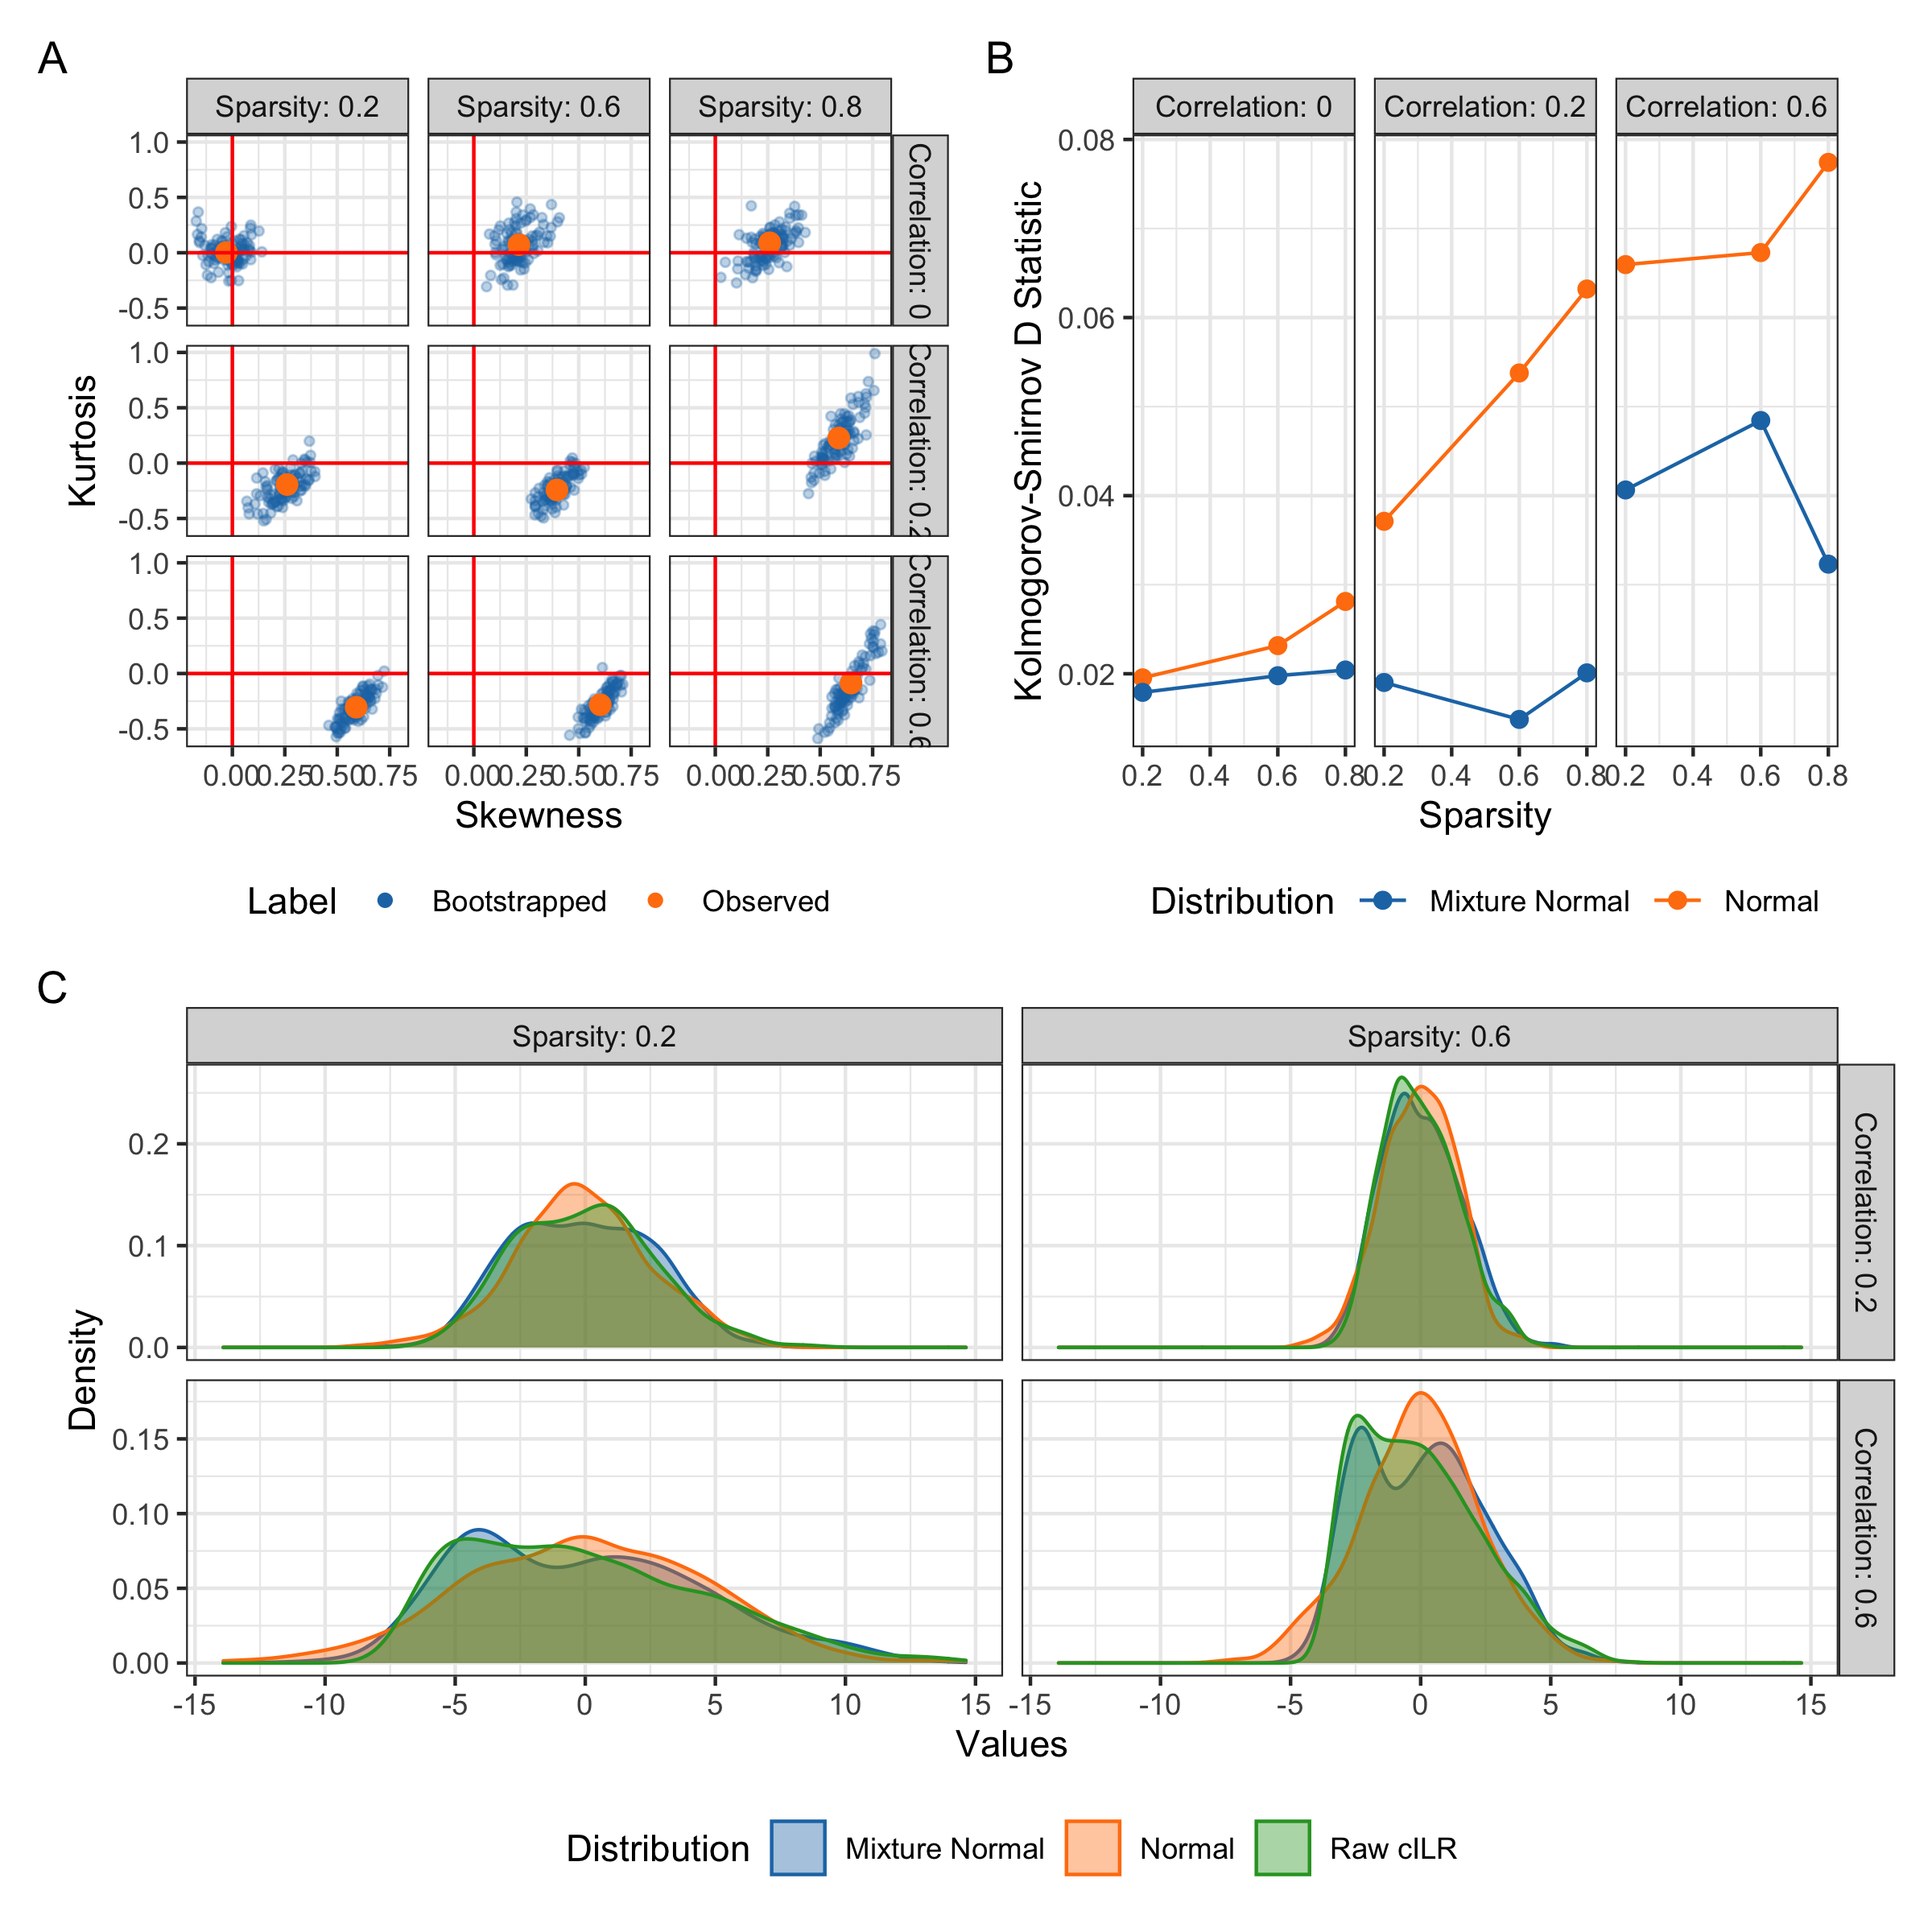
\includegraphics[width=\linewidth]{figures/kurtosis_skewness_gof.png}
    \caption{{\bf Properties of the null distribution of CBEA under the global null simulations}. Panel \textbf{(B)} presents kurtosis and skewness of CBEA scores while panel \textbf{(A)} presents the goodness of fit (as Kolmogorov-Smirnov D statistic) for mixture normal and normal distributions. Panel \textbf{(C)} is a density plot of the shape of the null distribution. Results indicated the necessity of estimating an empirical null and demonstrating that the mixture distribution was the better fit compared to the basic normal.}
    \label{fig:1}
\end{figure}

Additionally, the degree of kurtosis and skewness also suggests that the normal distribution itself might not be a good approximation of the null. To address this issue, we also evaluated a two-component normal mixture distribution. Panel B of Fig~\ref{fig:1} demonstrates the goodness of fit of the mixture normal and the normal distribution using Kolmogorov-Smirnov (KS) test statistic computed on fitted normal and mixture normal distribution when fitted on CBEA scores in simulation scenarios under the global null. We can see that the mixture normal distribution is a better fit (lower KS scores) than the normal distribution across both sparsity and correlation settings. 

We performed our empirical null estimation by fitting our distribution of choice and computing relevant parameters on raw CBEA scores on taxa-permuted data (equivalent to gene permutation in the gene expression literature). As such, the null distribution is characterized by scores computed on sets of equal size with randomly drawn taxa. 

\subsubsection*{Variance inflation due to inter-taxa correlation}  
When taxa within a set are highly correlated, the variance of the sample mean of taxon-wise statistics is inflated. Without loss of generalizability, for a set of taxa with taxa-specific statistics $x_1, ..., x_p$ we have the variance of the mean $\bar{x}$ to be:  
\begin{equation} \label{vareq:1}
    Var(\bar{x}) = \frac{1}{m^2}\left(\sum_{i = 1}(\sigma_i^2) + \sum_{i < j}\rho_{ij}\sigma_i\sigma_j\right)
\end{equation}
where $\sigma_i$ is the standard deviation of taxon $i$ while $\rho_{ij}$ is the correlation between $i$ and $j$. The second term of (\ref{vareq:1}) is the correlation dependent variance component, which goes to 0 if there is no correlation. The CBEA statistic follows a similar pattern. Since the geometric mean of a set of variables is equivalent to the exponential of the arithmetic mean of their logarithms, we can re-write CBEA score for a set $k$ with size $K$ as follows:  
\begin{equation}\label{vareq:2}
    M_{i,k} = \sqrt{\frac{K(p - K)}{K + (p - K)}} \left( \overbar{\log{X_{i,j|j \in K}}} - \overbar{\log{X_{i,j|j \notin K}}} \right)   
\end{equation}
where $p$ is the overall number of taxa, $j$ is the index of a taxa and $K$ is the set of indices of taxa in set $k$. The CBEA statistic then looks similar to a t-statistic for difference in means of log-transformed proportions. As such, the pooled variance of cILR is dependent on the variance inflation of both mean components $\overbar{\log{X_{i,j|j \in K}}}$ and $\overbar{\log{X_{i,j|j \notin K}}}$. The result of this variance inflation is inflated type I error since highly correlated sets are also detected as significantly enriched. 

However, as Wu et al. \cite{wu2012} showed, performing column permutation to estimate the null distribution of a competitive test statistic doesn't allow for adequate capture of this variance inflation factor since the permutation procedure disrupts the natural correlation structure of the original variables. It is important to address this problem since there is strong inter-taxa correlation within the microbiome \cite{kurtz2015a}. Our strategy for addressing issue is location (or mean) estimate from the column permuted raw score matrix with the spread (or variance) estimate from the original un-permuted scores. This still allows us to leverage the null generated via column permutation while using the proper variance estimate taken from scores where the correlation structure has not been disrupted. As such, this procedure assumes that the variance of the test statistic under the alternate hypothesis is the same as that of the null. Details of the computational implementation to this estimation process can be found in the Supplementary Materials.   

However, set-based analysis is an exploratory approach that can help generate functionally informative hypotheses, and as such users might not want strict type I error control in favor of higher power. This is especially true for competitive hypotheses, where its stricter formulation compared to the self-contained approach implies that the test naturally has lower power \cite{goeman2007, ackerman2009}. Furthermore, sets that are highly correlated compared to background can be biologically relevant. Therefore, CBEA provides an option for users to specify whether correlation adjustment is desired. 

\section*{Evaluation} \label{evaluation}
We based our evaluation strategy on gene set testing benchmarking standards set by Geistlinger et al. \cite{geistlinger2021} and utilized the same approaches whenever possible. All data sets are obtained from either the \emph{curatedMetagenomicData} \cite{pasolli2017} and \emph{HMP16SData} \cite{schiffer2019} R packages (2020-10-02 snapshot), or downloaded from the Qiita platform \cite{gonzalez2018}. All code and data sets used for evaluation of this method is publicly available and can be found on GitHub (\href{www.github.com/qpmnguyen/CBEA\_analysis}{qpmnguyen/CBEA\_analysis}). 

\subsection*{Statistical significance}
We evaluate the inference procedure of CBEA compared to alternate methods using two approaches: randomly sampled taxa sets and sample label permutation. These analyses were performed on the 16S rRNA gene sequencing of the oral microbiome from the Human Microbiome Project \cite{consortium2012, proctor2019}. This data set contains 369 samples split into two subsites: supragingival and subgingival. We processed this data set by removing all samples with total read counts less than 1000 and OTUs whose presence (at least 1 count) is in 10\% of samples or less.  

\subsubsection*{Sample-level inference} 
Due to CBEA's self-contained null hypothesis, we can perform inference at the sample level for the enrichment of a set. We evaluated this application by generating one random taxa of different sizes $S \in \{20, 50, 100, 150, 200\}$ across 500 iterations. Random sets can act as our estimate for type I error since this matches the CBEA null hypothesis stated in \nameref{methods}, where we expect within each sample sets of randomly sampled taxa should not be significantly enriched compared to the remainder background taxa. For this evaluation, we estimated type I error as the fraction of samples that detects our random set as significant at a p-value threshold of 0.05 with confidence bands computed from the standard error across all iterations.  Additionally, this analysis also demonstrate whether CBEA is sensitive to different set sizes.  

\subsubsection*{Population-level inference} 
We can perform enrichment testing at the population level by generating corresponding sample level CBEA scores and performing a two-sample test such as Welch's t-test. In order to evaluate CBEA under this context, we generated CBEA scores of sets representing genus-level annotation in above gingival data set \cite{consortium2012, proctor2019} and applied a t-test to test for enrichment (similar to GSVA \cite{hanzelmann2013}) across a randomly generated variable indicating case/control status (repeated 500 times). Type I error is estimated as the fraction of sets per iteration found to be significantly enriched with confidence bands computed from the standard error across all iterations. In addition, we also performed a random set analysis assessing, where we generated 100 sets of different set sizes $S \in \{20, 50, 100, 150, 200\}$ and evaluated the fraction of genera that were found to be differentially abundant across the original labels (supragingival versus subgingival subsite). 95\% confidence intervals were computed using the Agresti-Couli approach \cite{agresti1998}.  

\subsection*{Phenotype relevance}
We want to evaluate whether sets found to be significantly enriched by CBEA are relevant to the research question. To perform this assessment, we relied on the gingival data set mentioned prior \cite{consortium2012, proctor2019}. This data set was chosen due to its clear biological interpretation that can serve as the ground truth. Specifically, we expect aerobic microbes to be enriched in the supragingival subsite where the biofilm is exposed to the open air, while conversely anaerobic microbes thrive in the subgingival site \cite{thurnheer2016}. Genus-level annotations for microbial metabolism from Beghini et al. \cite{beghini2019} and was obtained from the GitHub repository associated with Calagaro et al. \cite{matteocalgaro2020}. For sample-level inference, we assessed power as the fraction of supragingival samples where aerobic microbes are significantly enriched. For population-level inference, power is the fraction of sets representing genus level taxonomic assignments were significant across subsite labels.  

In addition to statistical power, we also assessed phenotype relevance through evaluating whether highly ranked sets based on CBEA scores are more likely to be enriched according to ground truth. This is represented by the area under the receiving operator curve (AUROC/AUC) scores computed on CBEA scores against true labels (similar approach was used to evaluate VAM \cite{frost2020}). DeLong 95\% confidence intervals for AUC \cite{delong1988} were obtained for each estimate. 

\subsection*{Disease Prediction}
CBEA scores can also be used downstream analyses such as disease prediction tasks. We utilized two data sets for this evaluation: 

\begin{enumerate}
\item Whole genome sequencing of stool samples from inflammatory bowel disease (IBD) patients in the MetaHIT consortium \cite{nielsen2014}. This data set contains 396 samples from a cohort of European adults, where 195 adults were classified as having IBD (which includes patients diagnosed with either ulcerative colitis or Crohn's disease). We processed this data by removing all samples with less than 1,000 total read counts as well as any OTU who was present (at least 1 count) in 10\% of samples or less. Prior to model fitting, we back-transformed relative abundances into count data (to align the format with our 16S rRNA gene sequencing data set) using provided total number of reads aligned to MetaPhlan marker genes (per sample).   

\item 16S rRNA gene sequencing of stool samples from IBD patients in the pediatric RISK cohort \cite{gevers2014}. This data set contains 16S rRNA gene sequencing samples from a cohort of pediatric patients (ages $<$ 17) from the RISK cohort enrolled in the United States and Canada. Of the 671 samples obtained, 500 samples belong to patients with IBD. We processed this data set by removing all samples with less than 1,000 total read counts as well as any OTU who was present (at least 1 count) in 10\% of samples or less.   
\end{enumerate}

We evaluate disease prediction performance by fitting a random forest model \cite{breiman2001} using inputs as CBEA scores to classify samples of patients with IBD and healthy controls. Random forest was chosen as a baseline learner due to its flexibility as an out-of-the-box model that is easy to fit. In this instance we evaluated predictive performance of a default random forest model (without hyperparameter tuning) AUROC after 10-fold cross validation. Additionally, we utilized SMOTE to correct for class imbalances \cite{chawla2002}. Implementation was done using the \emph{tidymodels} suite of packages \cite{kuhn2020b}.   

\subsection*{Comparison Methods} 
We benchmarked the statistical properties of CBEA against existing baseline approaches. For sample-level inference analyses, utilized the Wilcoxon rank-sum test, which non-parametrically tests the difference in mean counts between taxa from a pre-defined set and its remainder similar to CBEA. For assessments at the population level, we compared CBEA against performing a standard test for differential abundance with set-level features generated via element-wise summations instead. We chose DESeq2 \cite{love2014} and corncob \cite{martin2020} since they represent both methods extrapolated from RNA-seq \cite{mcmurdie2014} and those developed specifically for microbiome data.   

Since disease prediction models and rankings-based phenotype relevance analyses seek to evaluate the informativeness of CBEA scores instead of relying on computing p-values, we compared performance against other single sample based approaches from the gene set testing literature, specifically ssGSEA \cite{barbie2009} and GSVA \cite{hanzelmann2013}. Additionally, for evaluating prediction, we also compared performance against a standard analysis plan where inputs are count-aggregated sets with the centered log-ratio (CLR) transformation. 

\section*{Results}
In this section, we present results for evaluating statistical significance, phenotype relevance, and predictive performance. In addition to real data, we also evaluated models based on parametric simulations, where results can be found in the Supplemental Materials.   

\subsection*{Statistical Significance}
\subsubsection*{Inference at the sample level}
CBEA provides significance testing at the sample level through a self-contained competitive null hypothesis. Generating random sets approximate the global null setting where within each sample, sets generated by randomly sampling taxa should not be significantly more enriched than remainder taxa.   

\begin{figure}[!h]
    \centering
    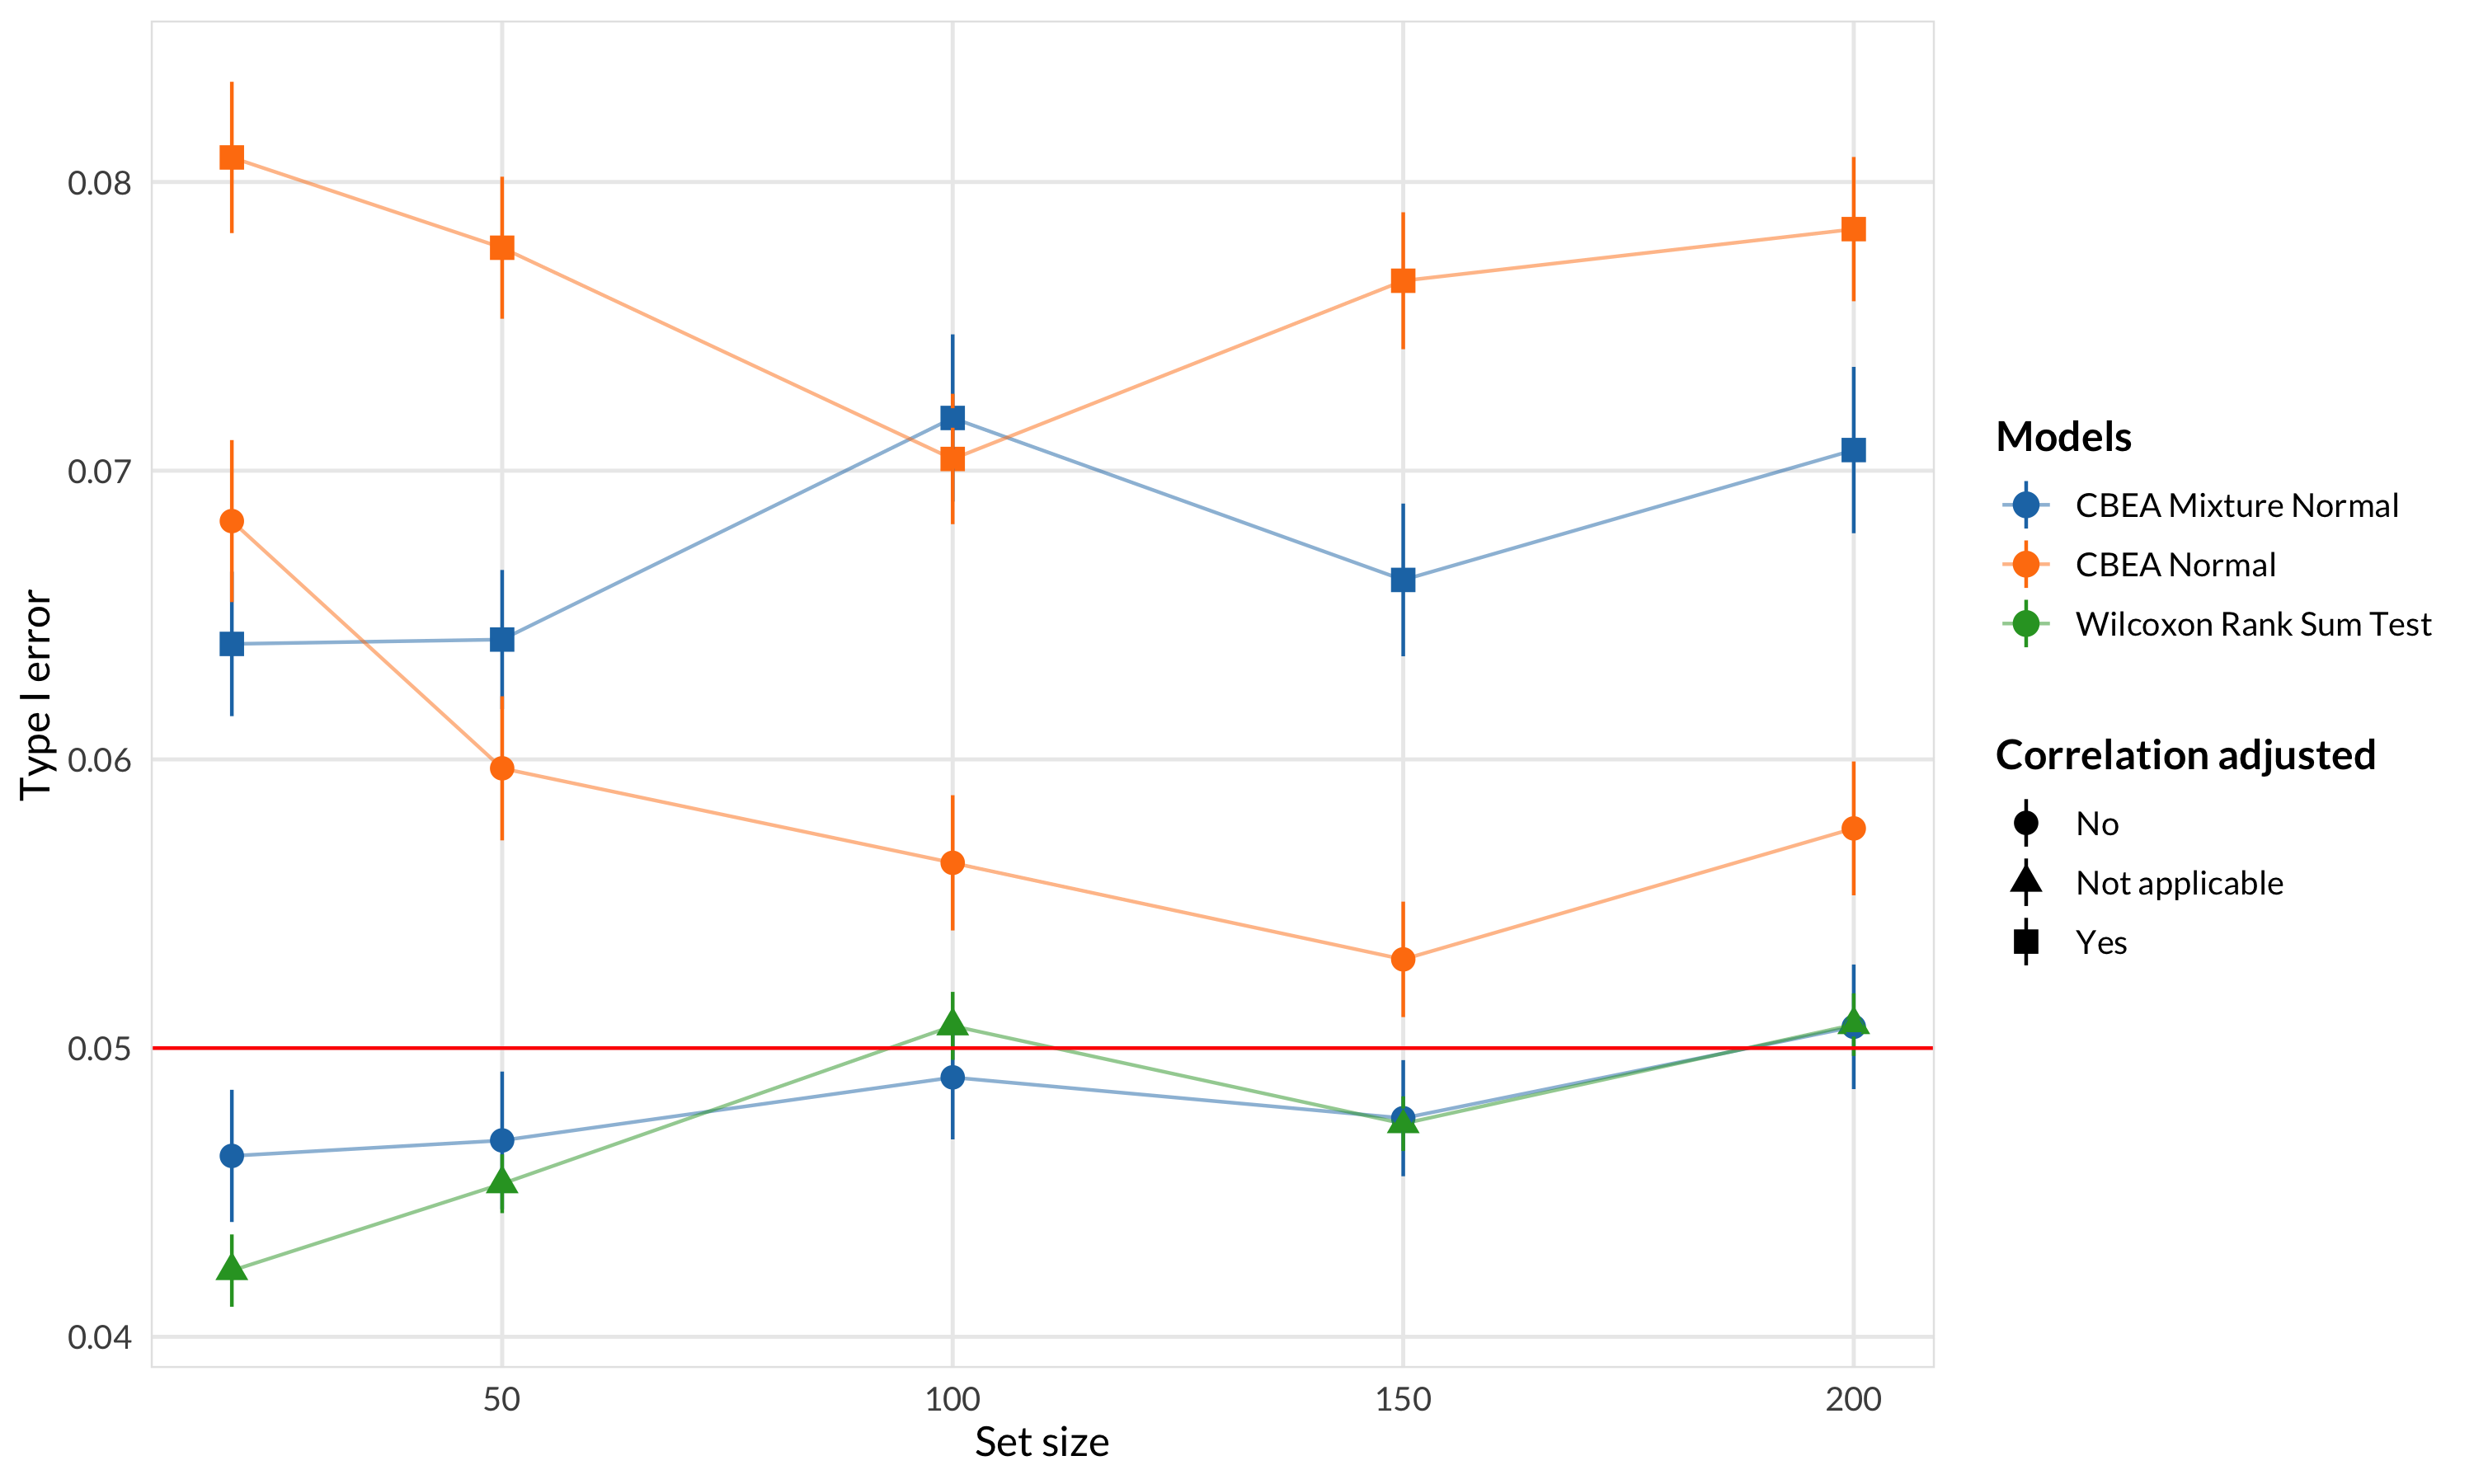
\includegraphics[width = \textwidth]{figures/data_ss_fdr_new.png}
    \caption{Random taxa set analyses for inference at the sample level of CBEA under different parametric assumptions compared against a Wilcoxon rank-sum test. Type I error (\emph{y}-axis) was evaluated by generating random sets of different sizes (\emph{x}-axis) (500 replications per size) and computing the fraction of samples where the set was found to be significantly enriched at $\alpha = 0.05$. Error bars represent the mean type I error $\pm$ sample standard error computed across 500 replications of the experiment.} 
    \label{fig:2}
\end{figure}

Fig~\ref{fig:2} demonstrates type I error of sample-level inference evaluated using the random set approach. The Wilcoxon rank sum test and unadjusted CBEA under mixture normal assumption demonstrated good type I error control at the appropriate $\alpha$ level. This fits with our expectations since the mixture normal distribution has much better fit than the normal distribution especially at the tails (Fig~\ref{fig:1}). However, other variants of CBEA demonstrated inflated type I error, especially correlation adjusted variants compared to their unadjusted counter parts. Encouragingly, all methods demonstrate consistent performance across all set sizes, with a slight increase in type I error at the highest levels.   

\subsubsection*{Inference at the population level}

Similar to other single sample approaches to gene set testing such as GSVA \cite{hanzelmann2013}, we can perform inference at the population level by utilizing a two-sample difference in means test. Here, we evaluate using CBEA scores generated under different settings with Welch's t-test in a supervised manner to assess whether a set is enriched across case/control status. 

\begin{figure}[!h]
    \centering
    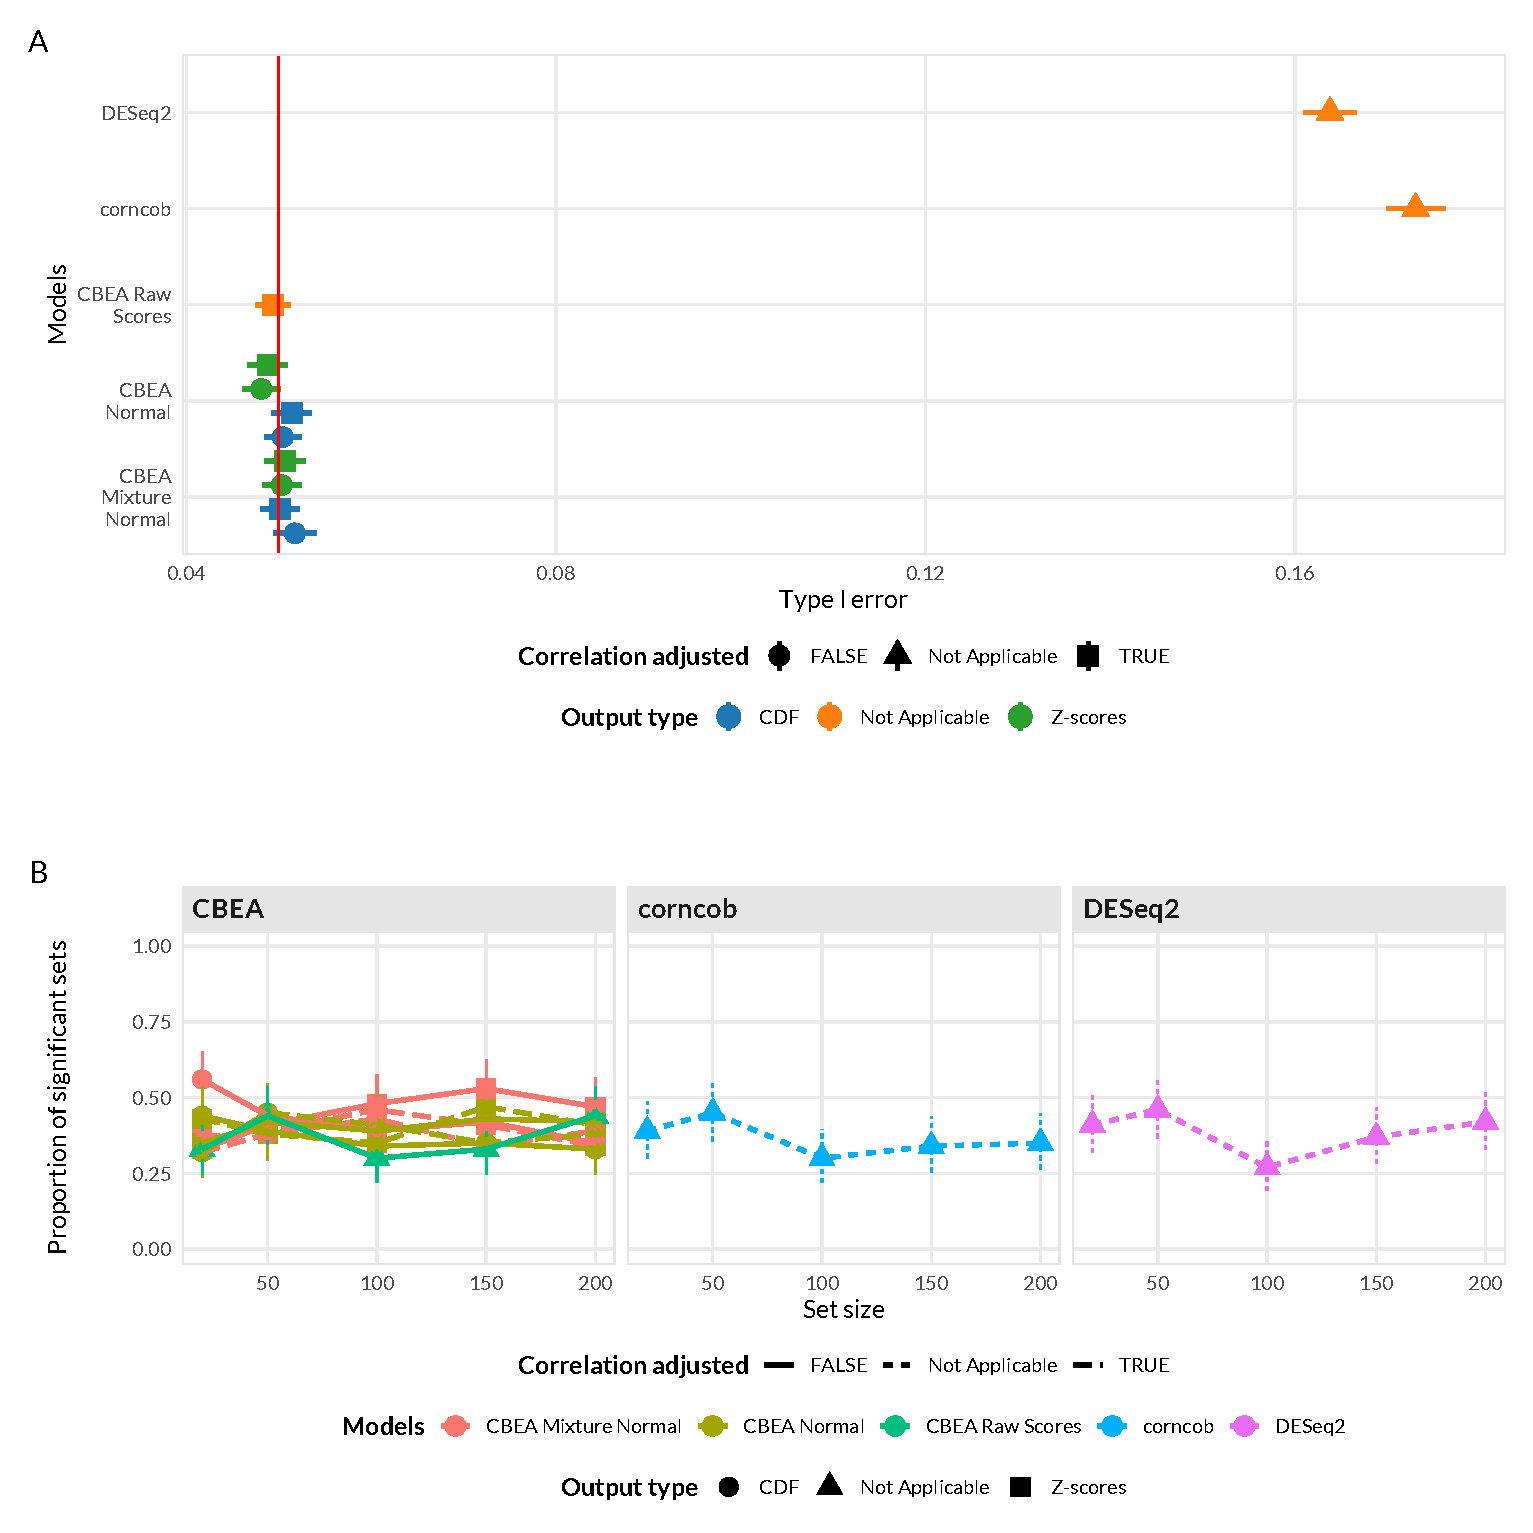
\includegraphics[width = \textwidth]{figures/data_diffab_fdr.eps}
    \caption{Random sample label (\textbf{A}) and random set (\textbf{B}) analyses for population level inference. (\textbf{A}) Type I error (\emph{x}-axis) was estimated as the overall fraction of sets found to be enriched $\alpha = 0.05$ using randomly generated sample labels (500 permutations).  Error bars represent the mean type I error $\pm$ sample standard error. (\textbf{B}) Proportion of significant sets (\emph{y}-axis) using 100 randomly generated sets of different set sizes (\emph{x}-axis). Confidence intervals computed using Agresti-Couli method for binomial proportions.}  
    \label{fig:3}
\end{figure}

Fig~\ref{fig:3} shows results for this scenario using both random sample label and random set evaluations. The random sample label approach (Fig~\ref{fig:3}A) provides a controlled setting where we can estimate type I error rate controlled at $\alpha = 0.05$. Across all replications, CBEA methods were able to control for type I error at the nominal threshold of 0.05, with CBEA raw scores being the most performant. Neither output types, correlation adjustment, nor distributional assumption improved performance values. Surprisingly, DESeq2 and corncob both exhibit significantly inflated type I error. 

We also assessed the impact of set-size on the inference procedure by testing for enrichment using the original sample labels but with randomly sampled sets of different sizes. Overall we observed very similar values across CBEA as well as corncob and DESeq2, suggesting that no individual method is systematically identifying too many significant sets. Additionally, similar to analogous analyses at the sample level, no approach were significantly sensitive to set-size. 

\subsection*{Phenotype Relevance} 
\subsubsection*{Inference at the sample level}
\begin{figure}[!h]
    \centering
    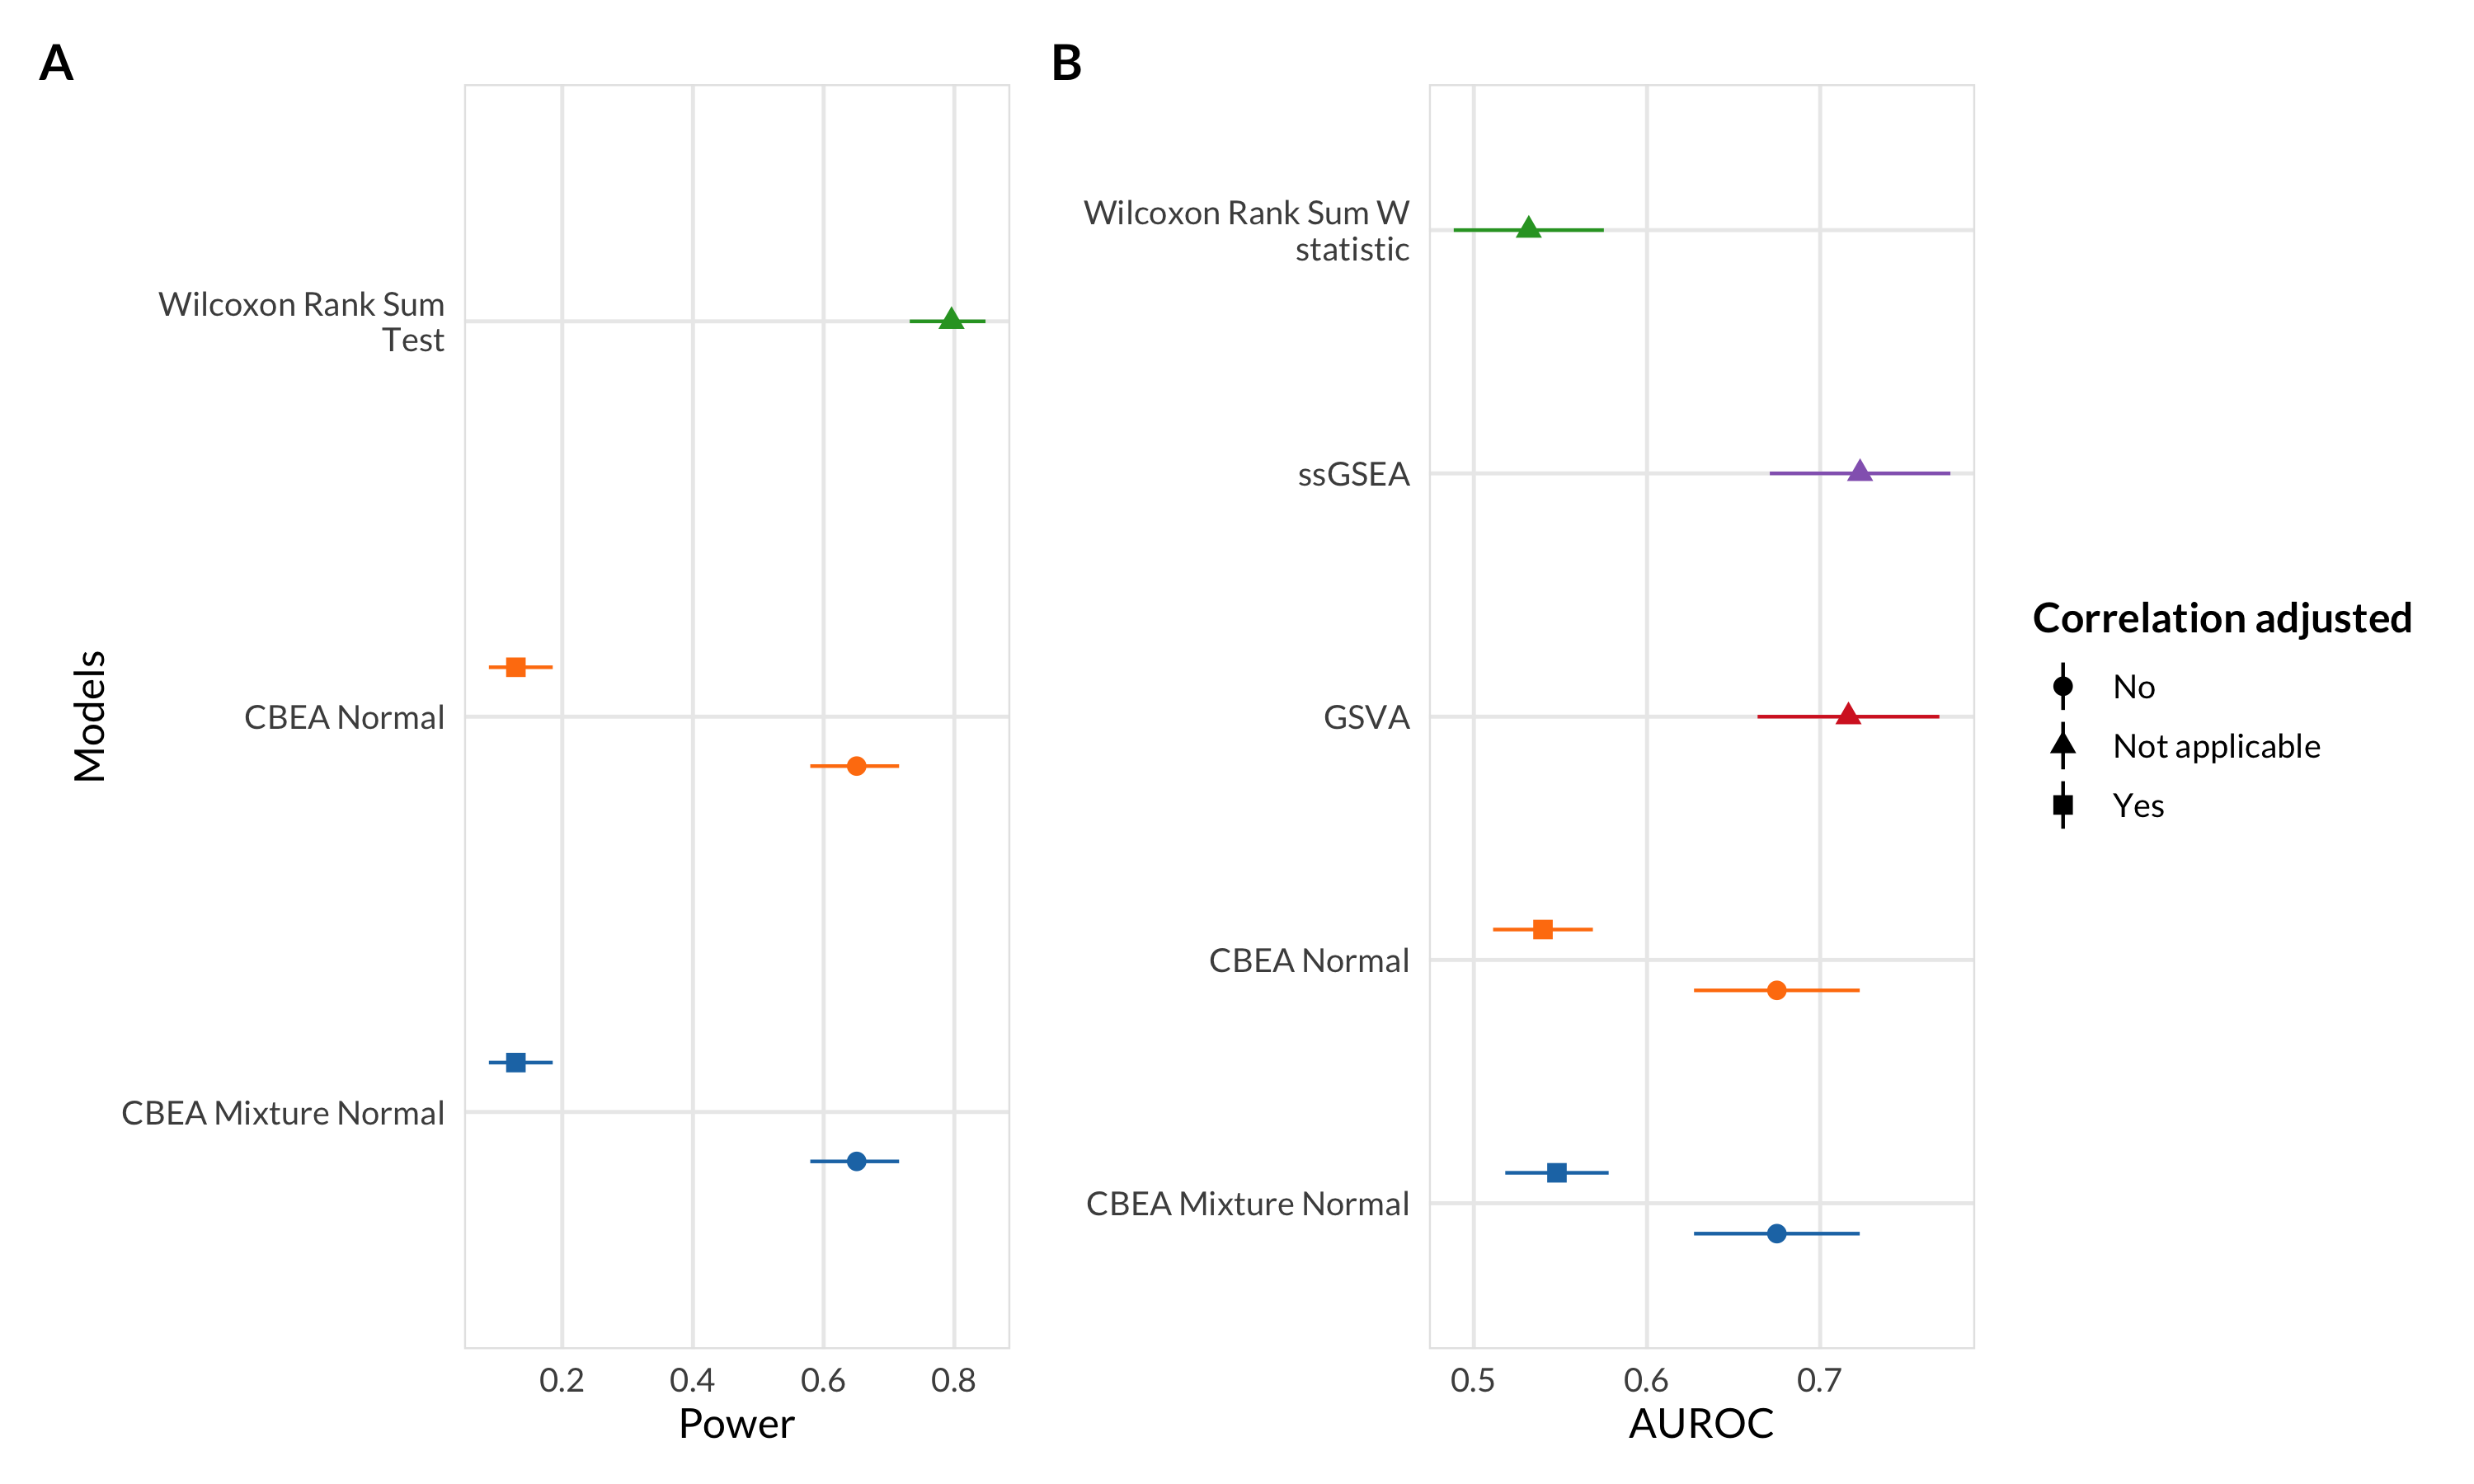
\includegraphics[width = \textwidth]{figures/data_ss_pwr_new.png}
    \caption{Statistical power (\textbf{A}) and score rankings (\textbf{B}) to assess phenotype relevance. (\textbf{A}) Power (\emph{x}-axis) was estimated as the overall fraction of aerobic microbes found to be enriched in supragingival samples at $\alpha = 0.05$. 95\% confidence intervals were computed using the Agresti-Couli approach for binomial proportions. (\textbf{B}) Score rankings were evaluated by comparing computed scores against true values using AUROC (\emph{x}-axis). DeLong 95 \% confidence intervals for AUROC were computed.} 
    \label{fig:4}
\end{figure}

In Fig~\ref{fig:4}, we evaluate whether sets found to be significant by CBEA are relevant to the phenotype of interest. We leveraged the gingival data set as stated in \nameref{evaluation} section where we know beforehand that aerobic microbes are more likely to be enriched in supragingival subsite samples and vice versa. 

We estimated statistical power using this data set as the fraction of supragingival samples where the set representing aerobic microbes were significantly enriched. We observed that adjusted CBEA approaches demonstrate much lower power compared to the Wilcoxon rank-sum test and unadjusted variants. This is surprising given the fact that in statistical significance analyses, the adjusted CBEA approach provides inflated type I error, especially if the normal distribution assumption was chosen. Here, we did not see any differences in performance between distribution choices. 

We also evaluated phenotype relevance by assessing whether enriched sets according to ground truth are preferentially ranked higher using assigned continuous scores (instead of performing a hypothesis test). This aspect is captured through computing AUROC values comparing computed enrichment scores and true labels. Consistent with prior approaches, adjusting for correlation did not improve performance, where the AUROC values are equivalent to using the Wilcoxon Rank sum statistic at around 0.5. Unadjusted methods were much better at ranking true enriched sets, however the mean AUROC values are lower than alternate single sample enrichment methods (GSVA \cite{hanzelmann2013} and ssGSEA \cite{barbie2009}) even though this difference is not significant due to overlapping confidence intervals.  

Unfortunately, evaluating power and score rankings using real data does not allow for observing performance trends when effect sizes, sparsity, and inter-taxa correlation are varied. In equivalent simulation analyses, we observed the opposite effect, where 

\subsubsection*{Inference at the population level}
\begin{figure}[!h]
    \centering
    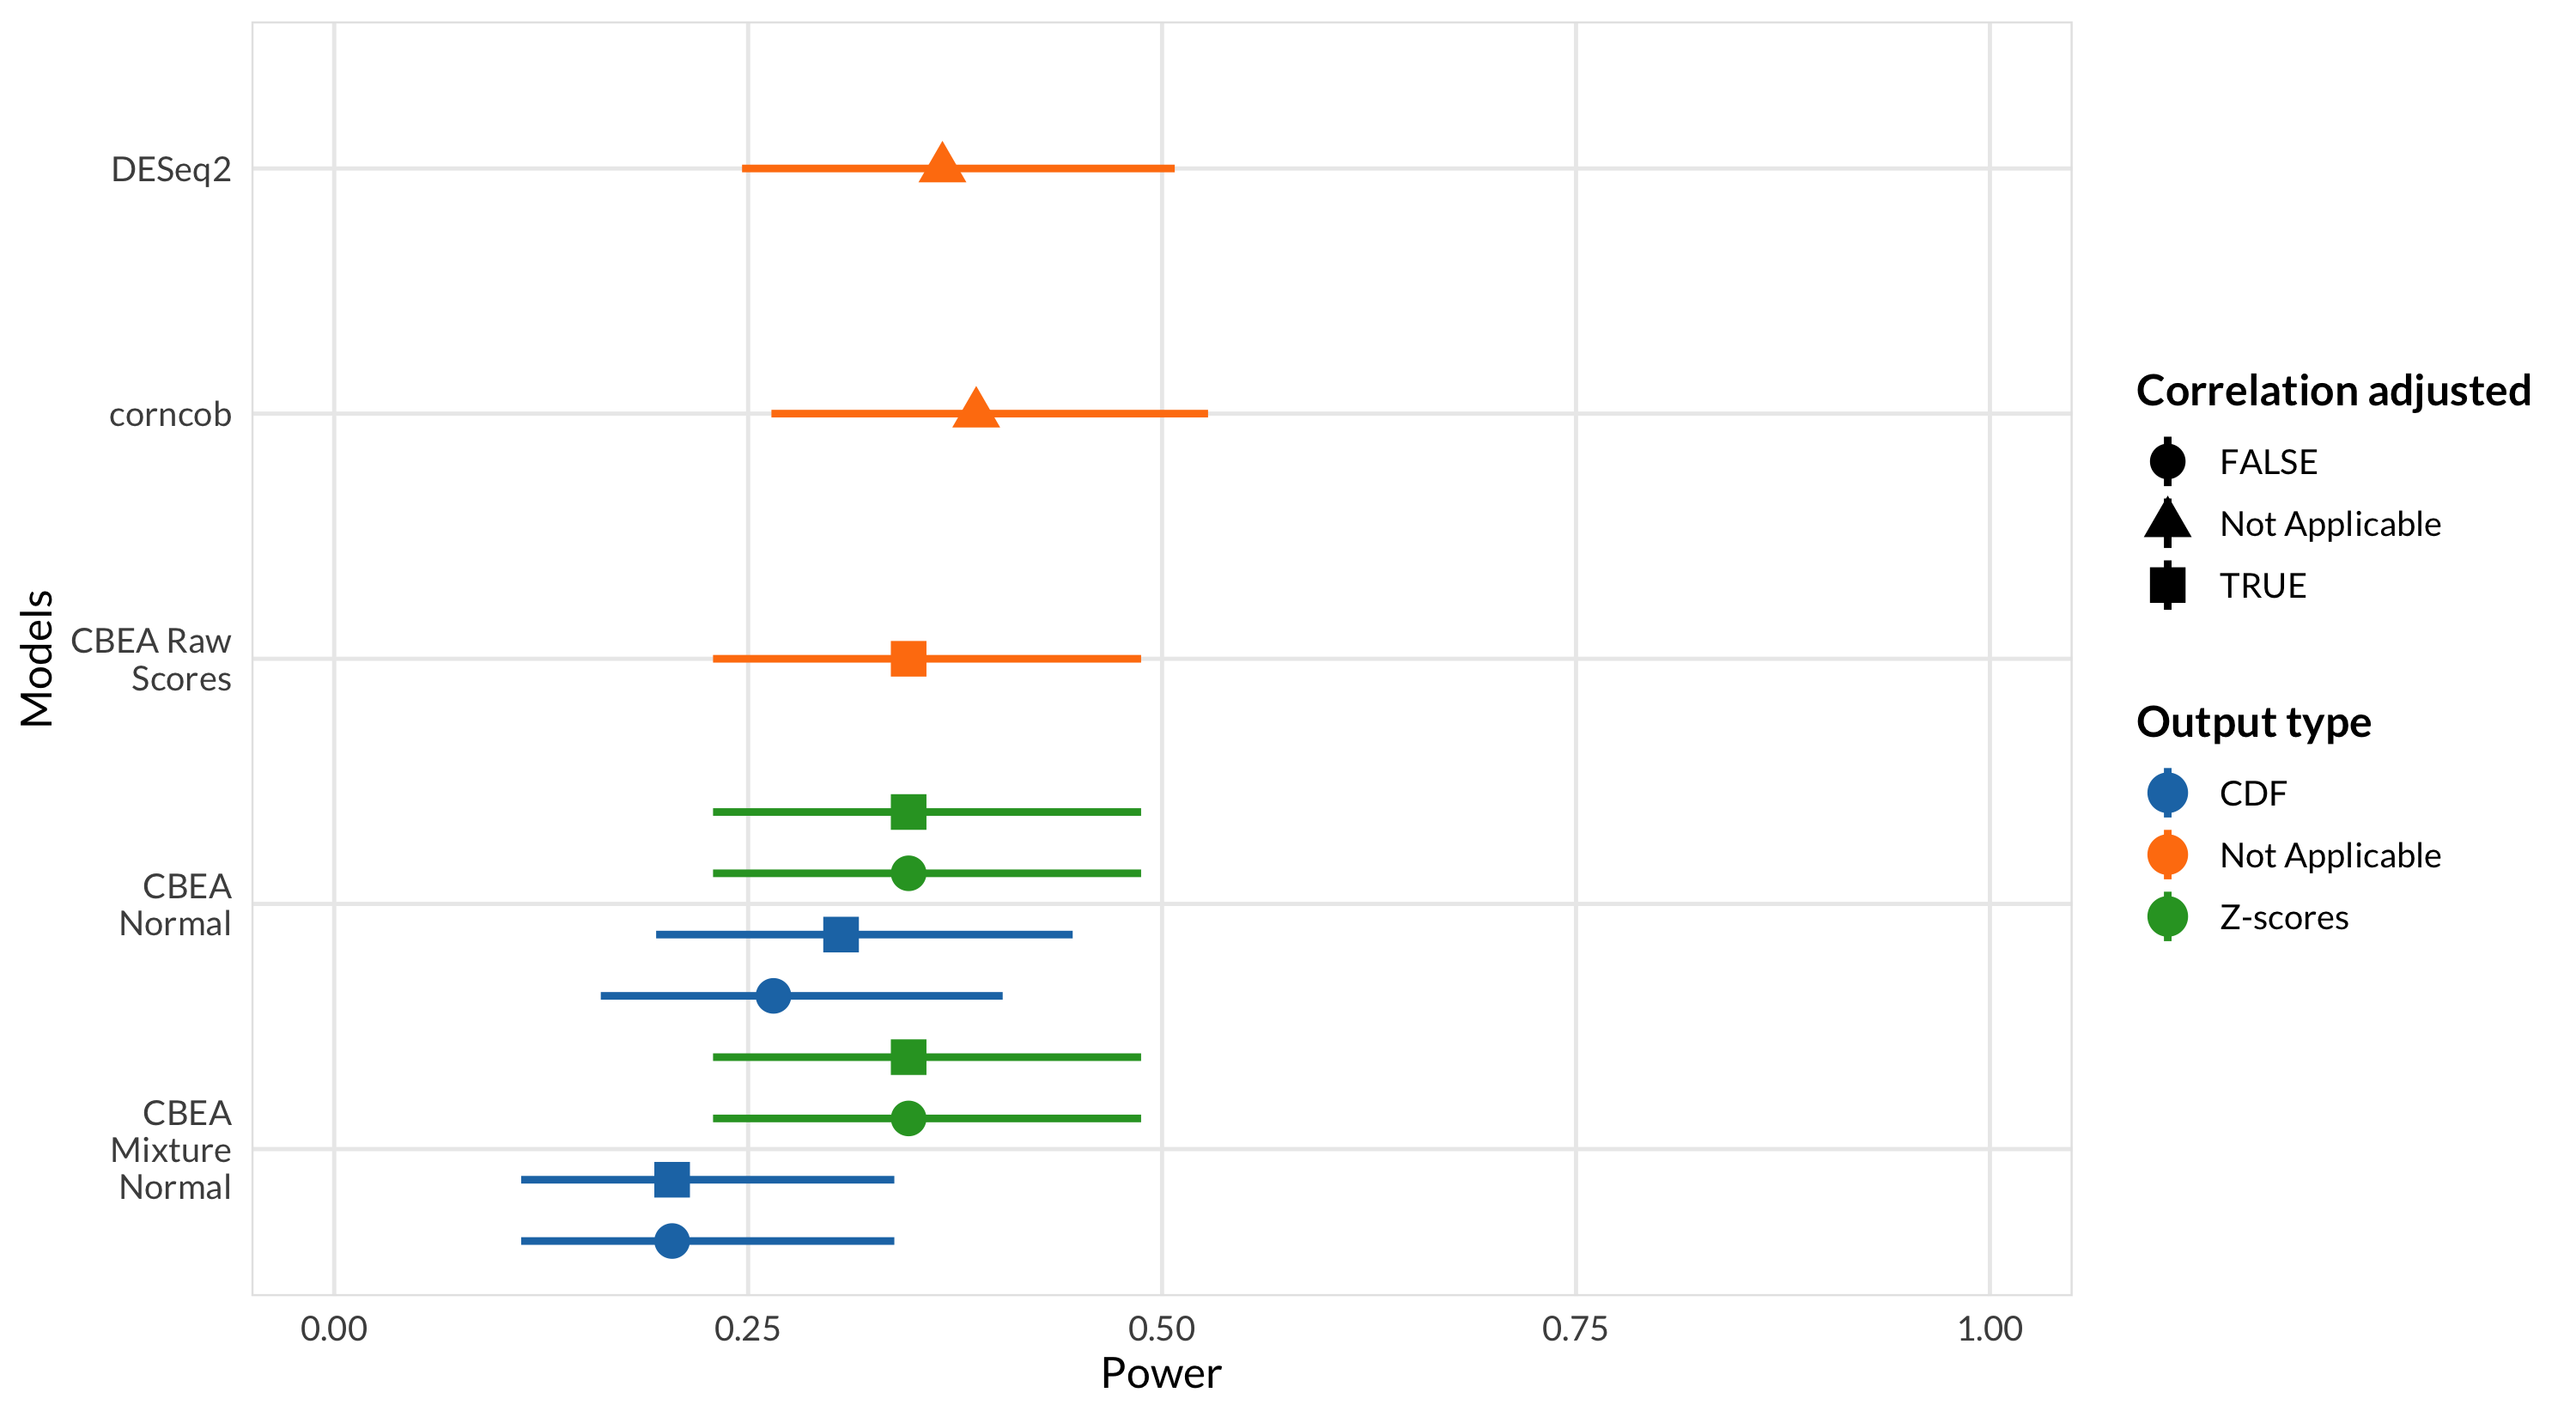
\includegraphics[width = \textwidth]{figures/data_diffab_pwr.png}
    \caption{Statistical power to assess phenotype relevance of inference tasks at the population level. Power (\emph{x}-axis) was estimated as the overall fraction of sets representing genera that are aerobic or anaerobic microbes found to be differentially enriched across sample type (supragingival or subgingival). 95\% confidence intervals were computed using the Agresti-Couli approach for binomial proportions.}  
    \label{fig:5}
\end{figure}

We also assessed statistical power for population level inference scenarios using a similar approach. Here, enrichment scores for sets representing all identified genera were computed, and estimated power as the fraction of sets found to be differentially enriched across sample site labels (supragingival or subgingival). We compared these results against performing a differential abundance test of genus level features generated via sum-based approaches. Results are shown in Fig~\ref{fig:5}. Some CBEA variants, such as CDF outputs for the mixture normal distributional assumption, did not correctly detect as many significant sets as DESeq2 or corncob despite very close performance values. Using raw CBEA scores was best approach, however it did not exceed values obtained from DESeq2 and corncob. 

\subsection*{Disease Prediction}   
Since CBEA can generate informative scores that can discriminate between samples with inflated counts for a set (Fig~\ref{fig:2}), we want to assess whether they can also act as useful inputs to predictive models. In this section we assessed the predictive performance of a standard baseline random forest model \cite{breiman2001} with different single sample enrichment scoring methods as inputs (evaluating CBEA, ssGSEA, and GSVA). Additionally, we also compared predictive performance of using these scores against the a standard approach of using the centered log ratio transformation (CLR) on taxon sets aggregated via abundance summations.     

%\begin{figure}[!ht]
%    \centering
%    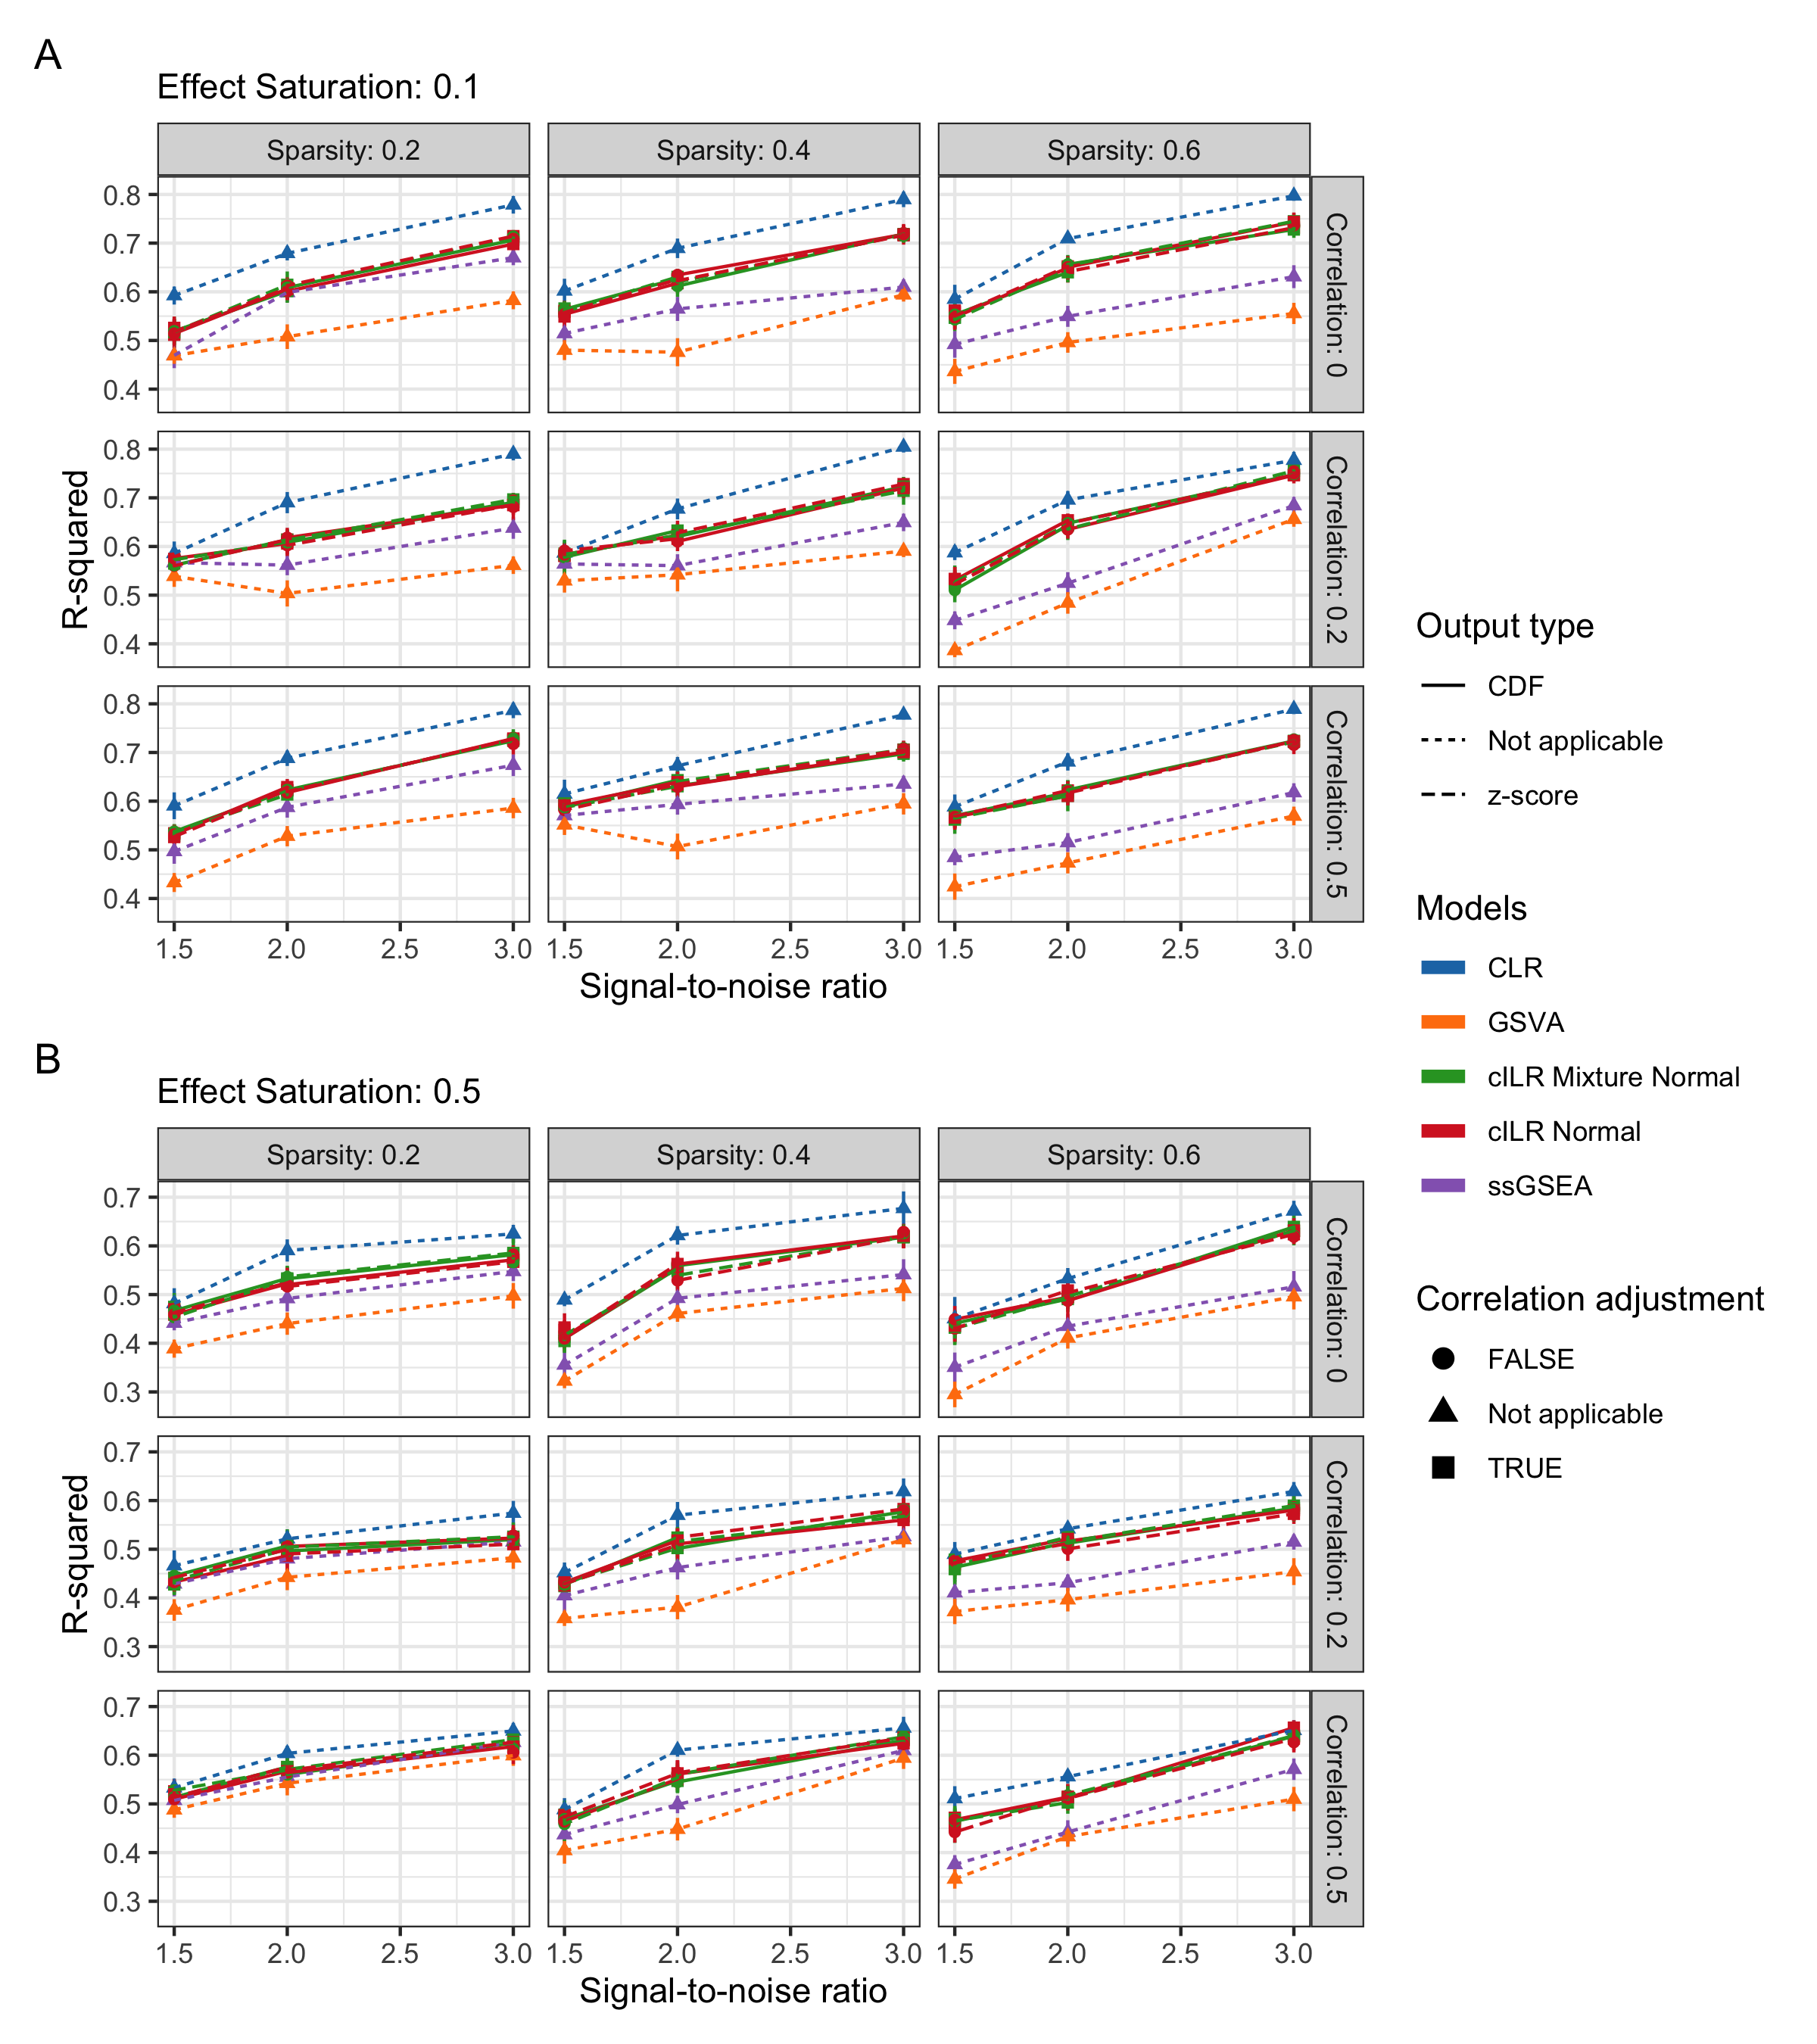
\includegraphics[width=\textwidth]{figures/sim_pred_rsq.png}
%    \caption{Predictive R-squared of a random forest model for a continuous outcome trained on CBEA,     %ssGSEA, GSVA generated scores as well as on standard CLR transformed data evaluated on simulated data %across sparsity levels, correlation, and signal-to-noise ratio. Panel \textbf{(A)} and \textbf{(B)} %represent results across different levels of model saturation (proportion of sets associated with the %outcome). CBEA approaches outperformed GSVA and ssGSEA but not standard CLR.}
%    \label{fig:sim_pred_rsq}
%\end{figure}

We fit our model to two data sets with a similar disease classification task of discriminating patients who are diagnosed with IBD (includes both Crohn's disease and ulcerative colitis) using only microbiome taxonomic composition. The two data sets represent different microbiome sequencing aprpaoches: the Gevers et al. \cite{gevers2014} data set uses 16S rRNA gene sequencing, while the Nielsen et al \cite{nielsen2014} data set uses whole genome shotgun sequencing. 

\begin{figure}[!h]
    \centering
    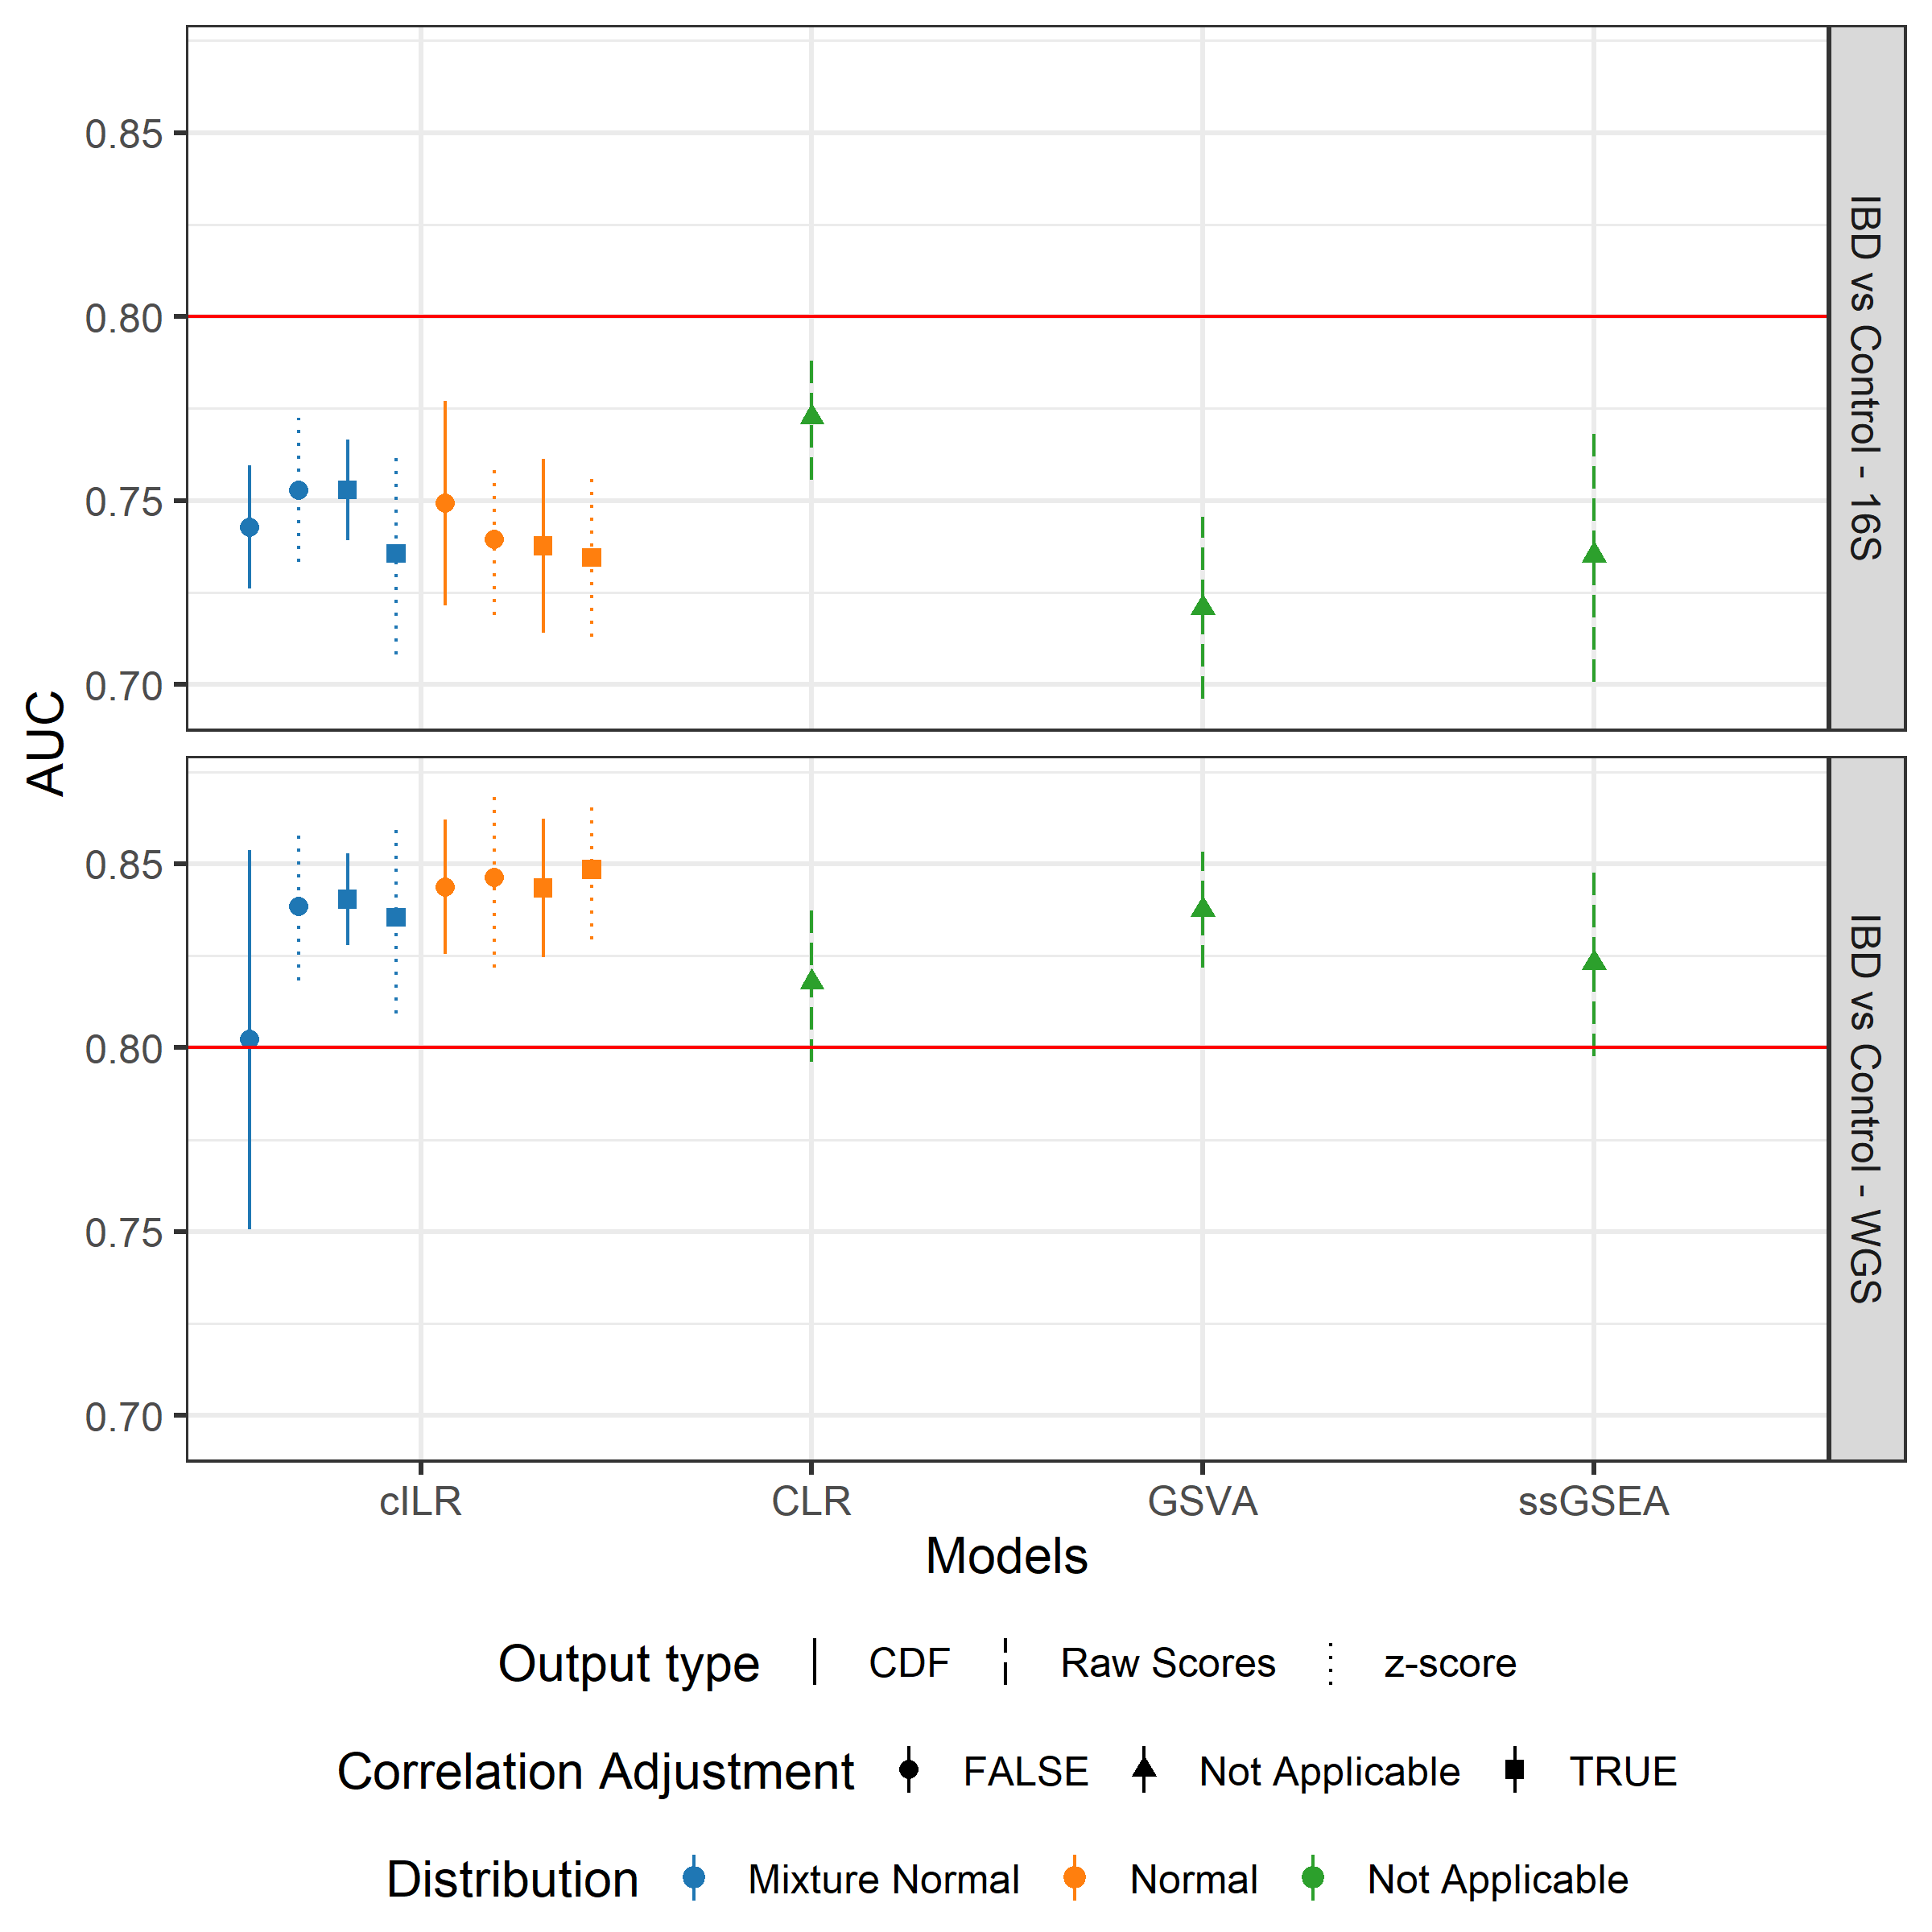
\includegraphics[width = \linewidth]{figures/data_prediction_plot.png}
    \caption{Predictive performance of a naive random forest model trained on CBEA, ssGSEA, GSVA generated scores as well as the standard CLR approach on predicting patients with inflammatory bowel disease versus controls using genus level taxonomic profiles. Data sets used span both 16S rRNA gene sequencing (Gevers et al. \cite{gevers2014}) and whole-genome shotgun sequencing (Nielsen et al. \cite{nielsen2014}). CBEA performs better than GSVA and ssGSEA but not as well as CLR, with the exception of the whole genome sequencing data set.}
    \label{fig:6}
\end{figure}

Fig~\ref{fig:6} illustrates results from using CBEA, ssGSEA, GSVA, or CLR transformed variables as inputs to our model, with AUROC as the performance criteria. Results also replicated that of the simulations (Supplementary materials), where across both data sets CBEA and CLR methods provide much better performance than both GSVA or ssGSEA. Interestingly, the CBEA approach performed better than CLR in the whole genome data set but did not perform as well in the 16S rRNA gene sequencing data set. However, these results indicate that CBEA generated scores are informative, providing competitive performance when acting as inputs to disease predictive models. Most importantly, performance values are consistent across both simulated and real data sets. 

These results demonstrate for given set-based features, CBEA can generate scores can could be informative in disease prediction tasks. Simulation results indicate that CBEA methods perform much better than either GSVA or ssGSEA, but not as well as the standard CLR approach. Interestingly, however, CBEA methods were much more competitive with CLR in either WGS data sets or data sets with higher sparsity levels. 

\section*{Discussion}

\subsection*{Inference with CBEA} 
CBEA is a microbiome-specific approach to generate sample specific enrichment scores for taxonomic sets defined apriori. The formulation of CBEA as a comparison between taxa within the set and its complement corresponds to the competitive null hypothesis in the gene set testing literature \cite{tian2005}. Since this null hypothesis is self-contained per sample, this allows users perform enrichment testing at the sample level. Additionally, in combination with a difference in means test, CBEA can also test for enrichment at the population level across case/control status similar to GSVA \cite{hanzelmann2013}.  

For single-sample analyses, we demonstrated that the CBEA approach (unadjusted with mixture normal parametric assumption) was able to control for type I error at the nominal level of 0.05 under the global null (Fig~\ref{fig:2}) while also demonstrating respectable power (Fig~\ref{fig:4}). This performance is consistent across different set sizes as well as our prior distributional fit analyses (Fig~\ref{fig:1}), where the mixture normal displayed superior fit to the null distribution. Unfortunately, other variants of CBEA did not demonstrate good type I error control. Interestingly, while the adjusted methods showed inflated type I error and low power in real data evaluations (Fig~\ref{fig:2}), they performed well in simulation studies (\nameref{S1_Fig}, \nameref{S3_Fig}). 

For population-level inference task, CBEA also performed very well. Under the permutation global null, representing genera abundance using CBEA scores in combination with Welch's t-test controls for type I error the correct $\alpha$ threshold while also showing respectable power. Since population level enrichment test is equivalent to differential abundance using set-based features, we compared CBEA approach against using element-wise summations with corncob \cite{martin2020} and DESeq2 \cite{love2014} to test for set-level differential abundance. We chose DESeq2 because it is an older approach from the bulk RNA-seq literature that has strong support for usage in microbiome taxonomic data \cite{mcmurdie2014}. Alternately, corncob is a newer method developed specifically for microbiome taxonomic data sets, where taxonomic counts are modeled directly using a beta-binomial distribution instead of relying on normalization via size factor estimation. We observed that using this approach resulted in an inflated type I error compared to all variants of CBEA (Fig~\ref{fig:2}), yet did not improve power (Fig~\ref{fig:4}). Results for CBEA approaches were replicated in simulation analyses, however for corncob and DESeq2 we observed an opposite effect: in simulation experiments, both methods show good type I error control but low power (\nameref{S2_Fig}, \nameref{S4_Fig}).  

We hypothesized that the discrepancy between simulation and real data evaluations can can arise due to differences in our assumptions regarding the data generating process that informed our simulation schema. One important consideration, as described in the \nameref{introduction} section, are taxon-specific biases that distort the observed relative abundance of taxa compred to true values \cite{mclaren2019}. In the context of sum-based aggregations, the resulting bias of the aggregated taxon are dependent on the relative abundances of the contributing taxa (Appendix I in \cite{mclaren2019}). Conceptually, this means that measurement error for a taxon aggregate is different across samples as relative abundance of contributing changes, leading to issues when attempting to perform inference. As such, we expect methods like corncob or DESeq2 when performed on such sum aggregates in the presence of taxon-specific biases to have inflated type I error compared to our taxon-ratio based approach. Conversely, in simulation studies, we did not explicitly include bias in our formulation and all taxa were generated from the same negative binomial distribution with similar variances across all samples (the only difference is when an enriched taxa is expected to have inflated means). As such, DESeq2 and corncob controls well for type I error in simulation scenarios where the effect of taxon-specific biases is absent. It is still surprising to see lower power for both methods in simulation analyses, which might be due to the fact that the evaluation protocol only considers default settings for both methods and did not attempt to optimize performance. We also suspect that 

\subsection*{Downstream analysis using predictive models}
The sample-level enrichment scores generated by the CBEA method can be used in downstream analyses such as disease prediction. Here, we evaluated whether CBEA can be used to generate set-based features for disease prediction models. 

We fitted a basic random forest model \cite{breiman2001} to predict continuous and binary outcomes using CBEA generated scores as inputs. Similar to our inference analysis, we compared CBEA against both ssGSEA and GSVA. Additionally, we also evaluated CBEA with the approach where counts of a set were aggregated using sums and applied the centered log-ratio transformation (CLR). This is because CLR is considered standard practice in using microbiome variables as predictors for a model \cite{gloor2017}. Results showed that CBEA generate scores perform well across both real data settings and simulation scenarios. Since predictive models consider the effect of variables jointly (and in the case of random forest, consider interactions as well), good performance indicates that CBEA scores can capture joint distribution of sets, enabling both uniset and multi-set type analyses. Comparatively, CBEA generated scores outperformed other enrichment score methods (GSVA and ssGSEA), suggesting that it is more tailored for microbiome taxonomic data sets. This is consistent with our sample ranking analysis (Fig~\ref{fig:3}), where CBEA scores are on average more informative when used to rank samples based on their propensity to have inflated counts. However, CBEA did not outperform the CLR approach across our simulation studies, and only marginally performed better in the real data analysis with WGS data. 

However, in simulation studies, this performance gap between CLR and CBEA decreases with higher sparsity and correlation, especially in low effect saturation scenarios. Additionally, there are also downsides to applying CLR. First, the singular covariance matrix of CLR transformed variables is singular due to a sum to zero constraint \cite{gloor2017}, preventing the proper usage of approaches that rely on matrix decomposition. Second, the procedure still relies on using summation of counts prior to transformation, which means that we still can't compare across sets of different sizes, and any bias might still be propagated \cite{mclaren2019}. As such, despite benefits in performance for a naive random forest model, there is still space for using CBEA as primary inputs into predictive models. 

\subsection*{Limitations and future directions} 

These above results demonstrate the applicability of CBEA under different data analysis scenarios. If researchers are interested in perform inference, they can decide between an unsupervised sample level approach (i.e. screen samples for enrichment of certain characteristics) or a supervised population level approach (i.e. identifying characteristics that are differentially abundant across case/control status). 

For the unsupervised approach, utilizing the unadjusted CBEA with the mixture normal distribution provides a good initial starting point. In the case where the screening procedure only wants to detect mean-inflated taxon sets (instead of additionally detecting taxon sets with increased correlation), users can apply the adjusted approach with the normal distribution, which can be effective at conserving type I error even at high correlation scenarios. However, the trade off for this adjustment is power that decreases with increasing correlation. For the supervised analysis, all CBEA variants control well for type I error and provides adequate statistical power. However, using raw CBEA scores with difference-in-means test such as Welch's t-test is preferable since it requires the least amount of computing resource (no estimation process) while still outperforming using sum-based approach with a standard differential abundance test.     

Beyond inference, CBEA scores are flexible and can be useful for downstream analysis. We demonstrated that for a given number of set-based features, CBEA can produce informative scores that contribute to competitive performance of prediction models even in low signal-to-noise ratios with high inter-taxa correlation and sparsity. This is especially true for whole genome sequencing data sets, where CBEA outperfrorms the standard approach of applying a centered log-ratio transformation. Even though we only evaluated prediction models in this manuscript, researchers can benchmark their own usage of CBEA for other downstream tasks such as sample ordination. 

However, there are various limitations to our evaluation of CBEA. First, our simulation analysis might not capture the appropriate data-generating distributions underlying microbiome taxonomic data. There is strong evidence to suggest that our zero-inflated negative binomial distribution is representative \cite{calgaro2020}, however other distributions such as the Dirichlet multinomial distribution \cite{wu2016a} have been used in the evaluation of prior studies. Second, we were not able to evaluate the phenotypical relevance of enrichment results as in Geistlinger et al. \cite{geistlinger2021} due to limited consistent annotations for microbiome signatures in health and disease, especially those that are experimentally verified (and not just from differential abundance studies). We attempted to perform this evaluation by leveraging the gingival data set similar to \cite{calgaro2020}. However, we acknowledge that this is not a perfect solution, since oxygen usage label of each microbe in the data set is only available at the genus level, and the difference in counts for obligate aerobes and anaerobes across the supragingival and subgingival sites might not be as clear cut. As such, results from power analyses using this data set is only relative between the comparison methods instead of treated as absolute measures of power or phenotype relevance. Finally, we assumed that taxa within a set are all equally associated with the outcome. This limits our ability to evaluate the performance of CBEA when only a small number of taxa within the set is associated with the outcome, or if there are variability in effect sizes or association direction of taxa within a set. 

Our evaluation also showed various drawbacks of the CBEA method itself. First, inference with CBEA at the sample level is limited, and can be affected by inter-taxa correlation if users wish to only detect mean-inflated sets, especially when inter-taxa correlation within the set is high. Second, for downstream analyses, CBEA might not always perform better than competing methods, especially when being used to generate inputs to predictive models. We hypothesized that this might be due to the lack of fit for the underlying null distribution in high correlation settings, especially the identifiability problem associated the estimation procedure associated with adjusting the mixture normal distribution. As such, we hope to refine the null distribution estimating procedure by either choosing a better distributional form, or to further constrain the optimization procedure of the mixture normal distribution by fixing the third and fourth moments. 

In addition, CBEA itself did not consider other aspects of microbiome data that can merit further extension. First, across all analyses, we relied on adding a pseudocount to ensure log operations are valid. Users can directly addressing this by incorporating model-based zero correction methods prior to modelling such as in \cite{martin-fernandez2012} or \cite{kaul2017a}. However, in our simulation studies, sparsity seems to not have a significant impact on the overall performance of our approach. Second, CBEA also treated all taxa within the set as equally contributing to the set. Incorporation of taxa-specific weights (similar to PhILR \cite{silverman2017} could reduce the influence of outliers, such as rare or highly invariant taxa. Finally, even though for a given set of apriori annotations CBEA can generate useful summary scores, such values are limited in their utility if the annotation themselves are not meaningful. As such, curating and validating sets (similar to MSigDB \cite{subramanian2005}) based on physiological or genomic characteristics of microbes \cite{weissman2021} or their association with human disease (in beta BugSigDB \url{https://bugsigdb.org/Main_Page}) can allow for incorporating functional insights into microbiome-outcome analyses.  

\section*{Conclusion}
Gene set testing, or pathway analysis is an important tool in the analysis of high-dimensional genomics data sets. However, limited work has been done developing set based methods specifically for microbiome relative abundance data. We introduced a new microbiome-specific method to generate set-based enrichment scores at the sample level. We demonstrated that our method can control for type I error for significance testing at the sample level, while generated scores are also valid inputs in downstream analyses, including disease prediction and differential abundance.  

\section*{Acknowledgments}
The authors thank Becky Lebeaux, Modupe Coker, Erika Dade, Jie Zhou, and Weston Viles for insightful comments and suggestions that greatly improved the paper. 

\nolinenumbers
% Either type in your references using
% \begin{thebibliography}{}
% \bibitem{}
% Text
% \end{thebibliography}
%
% or
%
% Compile your BiBTeX database using our plos2015.bst
% style file and paste the contents of your .bbl file
% here. See http://journals.plos.org/plosone/s/latex for 
% step-by-step instructions.
% 

\bibliography{mac_taxagg}{}
%\begin{thebibliography}{10}
%\end{thebibliography}



\section*{Supporting information}

% Include only the SI item label in the paragraph heading. Use the \nameref{label} command to cite SI items in the text.
\paragraph*{S1 Fig.}
\label{S1_Fig}
{\bf Computational performance of CBEA.} Computational time (in seconds) as a function of sample size (left panel) and number of taxa sets evaluated (right panel). Evaluation was performed on simulated data sets. For sample size analysis, only 10 sets were evaluated. For taxa set analysis, sample size was fixed at 1,000. Across all evaluations, the size of each taxa set was also fixed at 50. 

\paragraph*{S2 Fig.}
\label{S2_Fig}
{\bf Distribution of p-values.} Q-Q plot of 10,000 p-values compared against a uniform distribution bounded between 0 and 1. Evaluation was performed on simulated null data sets of 10,000 samples testing for enrichment of a set of size 50. For correlation of 0.5, p-values represent correlation adjusted CBEA while for correlation of 0, p-values represent unadjusted CBEA. 

\paragraph*{S3 Fig.}
\label{S3_Fig}
{\bf Computational performance of CBEA.} Computational time (in seconds) as a function of sample size (left panel) and number of taxa sets evaluated (right panel). Evaluation was performed on simulated data sets. For sample size analysis, only 10 sets were evaluated. For taxa set analysis, sample size was fixed at 1,000. Across all evaluations, the size of each taxa set was also fixed at 50. 

\paragraph*{S4 Fig.}
\label{S4_Fig}
{\bf Computational performance of CBEA.} Computational time (in seconds) as a function of sample size (left panel) and number of taxa sets evaluated (right panel). Evaluation was performed on simulated data sets. For sample size analysis, only 10 sets were evaluated. For taxa set analysis, sample size was fixed at 1,000. Across all evaluations, the size of each taxa set was also fixed at 50. 

\paragraph*{S5 Fig.}
\label{S5_Fig}
{\bf Computational performance of CBEA.} Computational time (in seconds) as a function of sample size (left panel) and number of taxa sets evaluated (right panel). Evaluation was performed on simulated data sets. For sample size analysis, only 10 sets were evaluated. For taxa set analysis, sample size was fixed at 1,000. Across all evaluations, the size of each taxa set was also fixed at 50. 

\paragraph*{S6 Fig.}
\label{S6_Fig}
{\bf Computational performance of CBEA.} Computational time (in seconds) as a function of sample size (left panel) and number of taxa sets evaluated (right panel). Evaluation was performed on simulated data sets. For sample size analysis, only 10 sets were evaluated. For taxa set analysis, sample size was fixed at 1,000. Across all evaluations, the size of each taxa set was also fixed at 50. 

\paragraph*{S7 Fig.}
\label{S7_Fig}
{\bf Computational performance of CBEA.} Computational time (in seconds) as a function of sample size (left panel) and number of taxa sets evaluated (right panel). Evaluation was performed on simulated data sets. For sample size analysis, only 10 sets were evaluated. For taxa set analysis, sample size was fixed at 1,000. Across all evaluations, the size of each taxa set was also fixed at 50. 

\paragraph*{S1 File.}
\label{S1_File}
{\bf Supplemental derivations.} Includes additional details on addressing variance inflation due to correlation in CBEA, as well as computational performance and p-value distribution of the method.   

\end{document}

